%------- ------- ------- Document Headers
\documentclass[10pt]{article} % latexmk, pdflatex
\usepackage[includefoot, paperheight=297mm, paperwidth=210mm, textwidth=170mm, textheight=257mm]{geometry} % texlive-geometry
\usepackage{lastpage} % texlive-lastpage
\usepackage{fancyhdr} % texlive-fancyhdr
\usepackage{graphicx} % 
\usepackage{indentfirst} % 
\usepackage{longtable} % 
\usepackage{array} % 
\usepackage{multicol} % 
\usepackage{multirow} % texlive-multirow
\usepackage{enumitem} % texlive-enumitem
\usepackage{mathtools} % texlive-mathtools
\usepackage{amsfonts} % texlive-amsfonts
\usepackage{amssymb} % 
\usepackage{hyperref} % texlive-hyperref
\usepackage{titlesec} % texlive-titlesec
\usepackage{tikz} % 
\usepackage{tkz-euclide} % texlive-tkz-euclide
%------- ------- ------- Initialization
\setlength{\parindent}{32pt}
\renewcommand{\baselinestretch}{0.7}
\renewcommand{\contentsname}{Sumário}
%------- ------- fancyhdr
\pagestyle{fancy}
\fancyhf{}
\renewcommand{\headrulewidth}{0pt}
\fancyfoot[R]{\thepage \hspace{1pt} / \pageref*{LastPage}}
%------- ------- array
\renewcommand{\arraystretch}{2}
%------- ------- multicol
\setlength{\columnsep}{32pt}
%------- ------- enumerate
\setlist{noitemsep, itemindent=64pt, labelwidth=0pt}
%------- ------- hyperref
\hypersetup{colorlinks=true, linkcolor=blue, pdfpagemode=FullScreen, pdftitle={Annotationes Meae}, pdfauthor={Gustavo Aragão}}
%------- ------- titlesec
\titleformat{\section}[block]{\normalfont\Large\bfseries}{\thesection}{16pt}{}
\titleformat{\subsection}[block]{\normalfont\large\bfseries}{\hspace{16pt}\thesubsection}{16pt}{}
\titleformat{\subsubsection}[block]{\normalfont\bfseries}{\hspace{32pt}\thesubsubsection}{16pt}{}
%------- ------- tikz
\usetikzlibrary{matrix}
\pgfdeclarelayer{bg}
\pgfdeclarelayer{fg}
\pgfsetlayers{bg,main,fg}
%------- ------- Commands
\newcommand{\eg}{\textit{e.g.:}}
%------- ------- ------- Beginning of Document
\begin{document}
    %------- ------- Title
    \title{
        \begin{tikzpicture}[scale=0.3, line join=bevel]
            % \a and \b are two macros defining characteristic
            % dimensions of the Penrose triangle.		
            \pgfmathsetmacro{\a}{2.5}
            \pgfmathsetmacro{\b}{0.9}
    
            \tikzset{
              apply style/.code     = {\tikzset{##1}},
              triangle_edges/.style = {thick,draw=black}
            }
    
            \foreach \theta/\facestyle in {
                0/{triangle_edges, fill = gray!50},
                120/{triangle_edges, fill = gray!25},
                240/{triangle_edges, fill = gray!90}
            }{
                \begin{scope}[rotate=\theta]
                    \draw[apply style/.expand once=\facestyle]
                    ({-sqrt(3)/2*\a},{-0.5*\a})                     --
                    ++(-\b,0)                                       --
                    ({0.5*\b},{\a+3*sqrt(3)/2*\b})                -- % higher point	
                    ({sqrt(3)/2*\a+2.5*\b},{-.5*\a-sqrt(3)/2*\b}) -- % rightmost point
                    ++({-.5*\b},-{sqrt(3)/2*\b})                    -- % lower point
                    ({0.5*\b},{\a+sqrt(3)/2*\b})                  --
                    cycle;
                \end{scope}
            }	
        \end{tikzpicture} \\
        \vspace{8pt} Annotationes Meae \\ Mathematicae
    }
    \author{\textit{Gustavo Aragão}}
    \date{}
    \maketitle
    \thispagestyle{fancy}
    %------- ------- Table of Contents
    \tableofcontents
    \newpage
    %------- ------- 1
    \section{Lógica e Notação}
    %------- 1.1
\subsection{Conectivos}
    \begin{center}
        \begin{longtable}{| m{3cm} | m{12cm} |}
                \hline $ \neg $ & Negação\\
                \hline $ \vee $ & Disjunção\\
                \hline $ \wedge $ & Conjunção\\
                \hline $ \rightarrow $ & Implicação; Condicional\\
                \hline $ \leftrightarrow $ & Bi-implicação; Equivalência\\
                \hline
            \end{longtable}
    \end{center}
%------- 1.2
\subsection{Quantificadores}
    \begin{center}
        \begin{longtable}{| m{3cm} | m{12cm} |}
            \hline $ \forall $ & Todo; Qualquer\\
            \hline $ \exists $ & Existe; Pelo menos um; Algum\\
            \hline $ \exists ! $ & Existe exatamente um\\
            \hline
        \end{longtable}
    \end{center}
%------- 1.3
\subsection{Pontuações}
    \begin{center}
        \begin{longtable}{| m{3cm} | m{12cm} |}
            \hline $ \pm $ & Mais ou menos\\
            \hline $ = $ & Igual\\
            \hline $ \neq $ & Diferente\\
            \hline $ \equiv $ & Equivalente; Congruente\\
            \hline $ \sim $ & Aproximadamente\\
            \hline $ \approx $ & Aproximadamente igual\\
            \hline $ > $ & Maior que\\
            \hline $ \geq $ & Igual ou maior que\\
            \hline $ < $ & Menor que\\
            \hline $ \leq $ & Igual ou menor que\\
            \hline $ \star $ & Igual, maior ou menor que\\
            \hline $ \prec $ & Sequencialmente precede\\
            \hline $ \succ $ & Sequencialmente sucede\\
            \hline $ \propto $ & Proporcional\\
            \hline $ | $ & Tal que\\
            \hline $ ( ), [ ], \{ \} $ & Delimitadores\\
            \hline $ (\cdots)_p $ & Enupla de $p$ elementos\\
            \hline $ \{\cdots\} $ & Conjunto\\
            \hline $ \varnothing, \{\} $ & Conjunto vazio\\
            \hline $ \# $ & Número de elementos contidos\\
            \hline $ \nexists $ & Não existe\\
            \hline $ \ni, \supset $ & Contém\\
            \hline $ \not\ni, \not\supset $ & Não contém\\
            \hline $ \in, \subset $ & Está contido\\
            \hline $ \notin, \not\subset  $ & Não está contido\\
            \hline $ \supset $ & É subconjunto\\
            \hline $ \subset $ & É superconjunto\\
            \hline $ \cup $ & União\\
            \hline $ \cap $ & Interseção\\
            \hline $ \mathcal{P} $ & Propriedade; Lei de aplicação\\
            \hline $ \mathcal{D} $ & Domínio\\
            \hline $ \mathcal{CD} $ & Contradomínio\\
            \hline $ \mathcal{IM} $ & Imagem\\
            \hline $ \mathcal{C}^{B}_{A} $ & Complementar de $B$ em $A$\\
            \hline $ A^* $ & Conjunto dos elementos não nulos de $A$\\
            \hline $ A^n $ & Conjunto dos $n$ primeiros elementos de $A$\\
            \hline $ A_+ $ & Conjunto dos elementos positivos de $A$\\
            \hline $ A_- $ & Conjunto dos elementos negatios de $A$\\
            \hline $ \mathbb{N} $ & Conjunto dos números naturais\\
            \hline $ \mathbb{Z} $ & Conjunto dos números inteiros\\
            \hline $ \mathbb{Q} $ & Conjunto dos números racionais\\
            \hline $ \mathbb{I} $ & Conjunto dos números irracionais\\
            \hline $ \mathbb{R} $ & Conjunto dos números reais\\
            \hline $ \mathfrak{I} $ & Conjunto dos números imaginários\\
            \hline $ \mathbb{C} $ & Conjunto dos números complexos\\
            \hline $ \mathbb{U} $ & Conjunto universo\\
            \hline $ \mapsto $ & Função aplicada\\
            \hline $ \mathrm{P}(n) $ & Polinômio de Grau $n$\\
            \hline $ \therefore $ & Portanto\\
            \hline $ \because $ & Em razão de\\
            \hline $ \infty $ & Infinito\\
            \hline $ \Delta $ & Variação\\
            \hline $ \lim\limits_{a \to b} f(x) $ & Limite\\
            \hline $ f', \frac{dy}{dx} $ & Derivada\\
            \hline $ \frac{\partial y}{\partial x}  $ & Derivada parcial\\
            \hline $ \int_a^b $ & Integral\\
            \hline $ \oint_a^b $ & Integral de linha\\
            \hline $ \nabla $ & Gradiente\\
            \hline $ \displaystyle\sum_{i=a}^{b} f(i) $ & Somatório\\
            \hline $ \displaystyle\prod_{i=a}^{b} f(i) $ & Produtório\\
            \hline $ \mathring{APB} $ & Ponto $P$ contido entre $A$ e $B$\\
            \hline $ \overline{AB} $ & Segmento de reta\\
            \hline $ \overrightarrow{AB} $ & Semirreta\\
            \hline $ \hat{\alpha}, \hat{AOB} $ & Ângulo\\
            \hline $ \parallel $ & Paralelo\\
            \hline $ \nparallel $ & Concorrente\\
            \hline $ \bot $ & Perpendicular\\
            \hline $ \triangle ABC $ & Triângulo ABC\\
            \hline $ \Diamond ABCDE $ & Polígono ABCDE\\
            \hline
        \end{longtable}
    \end{center}
%------- 1.4
\subsection{Alfabeto Grego}
    \begin{center}
        \begin{longtable}{| m{3cm} | m{3cm} | m{8.57cm} |}
            \hline $ \alpha $ & $ A $ & Alfa\\
            \hline $ \beta $ & $ B $ & Beta\\
            \hline $ \gamma $ & $ \Gamma $ & Gama\\
            \hline $ \delta $ & $ \Delta $ & Delta\\
            \hline $ \epsilon $ & $ E $ & Epsilon\\
            \hline $ \zeta $ & $ Z $ & Zeta\\
            \hline $ \eta $ & $ H $ & Eta\\
            \hline $ \theta $ & $ \Theta $ & Theta\\
            \hline $ \iota $ & $ I $ & Iota\\
            \hline $ \kappa $ & $ K $ & Kappa\\
            \hline $ \lambda $ & $ \Lambda $ & Lambda\\
            \hline $ \mu $ & $ M $ & Mu\\
            \hline $ \nu $ & $ N $ & Nu\\
            \hline $ \xi $ & $ \Xi $ & Xi\\
            \hline $ o $ & $ O $ & Omicron\\
            \hline $ \pi $ & $ \Pi $ & Pi\\
            \hline $ \rho $ & $ P $ & Rho\\
            \hline $ \sigma $ & $ \Sigma $ & Sigma\\
            \hline $ \tau $ & $ T $ & Tau\\
            \hline $ \upsilon $ & $ \Upsilon $ & Upsilon\\
            \hline $ \phi $ & $ \Phi $ & Phi\\
            \hline $ \chi $ & $ X $ & Chi\\
            \hline $ \psi $ & $ \Psi $ & Psi\\
            \hline $ \omega $ & $ \Omega $ & Omega\\
            \hline
        \end{longtable}
    \end{center}
    %------- ------- 2
    \section{Teoria dos Conjuntos}
    %------- 2.1
\subsection{Conceitos Básicos}
    %--- 2.1.1
    \subsubsection{Definição}
        Conjunto é um agrupamento de elementos, aleatórios ou selecionados criteriosamente por um sistema. Pode ser enumerado ou ter seus critérios descritos em propriedades. \eg
        \[ A = \{ 0,1,2,3,5,8,13 \}; A = \{ x \in \mathbb{U} | \mathcal{P} \} \]
    %--- 2.1.2
    \subsubsection{Tipos}
        \begin{description}
            \item[Conjunto Unitário] é aquele que possui um único elemento. \eg \hfill $ A = \{7\} $
            \item[Conjunto Vazio] é aquele que não possui elemento algum. \eg \hfill $ A = \{  \}; A = \varnothing $
            \item[Conjunto Universo] é aquele que contém todos os elementos utilizados no assunto
tratado
        \end{description}
    %--- 2.1.3
    \subsubsection{Intervalos}
        Definido como uma descrição de conjunto que compreende todos os números em determinado espaço da reta numérica (considerado o conjunto universo), podendo ser abertos ou fechados. \eg
        \[ (a<b) \]
        \[ ]a,b[ = \{ x \in \mathbb{U} | a < x < b \} \]
        \[ [a,b] = \{ x \in \mathbb{U} | a \leq x \leq b \} \]
        
        Intervalos possuem uma representação gráfica na reta numérica. \eg
        \begin{center}
            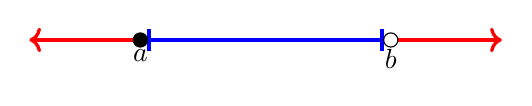
\begin{tikzpicture}
                \draw[red, very thick, <->] (-3,0) -- (3,0);
                \draw[blue, very thick, |-|] (-1.5,0) -- (1.5,0);
                \filldraw[color=black, fill=black] (-1.59,0) circle (0.09) node[below]{$a$};
                \filldraw[color=black, fill=white, thin] (1.59,0) circle (0.09) node[below]{$b$};
            \end{tikzpicture}
            \[ [a,b[ = \{ x \in \mathbb{R} | a \leq x < b \} \]
        \end{center}
    %--- 2.1.4
    \subsubsection{Pares Ordenados}
        Chama-se par ordenado o conjunto de 2 elementos onde sua ordem importa:
        \[ (a,b) = \{ \{ a \}, \{ a, b \} \} \]
        \[ (a,b) = (c,d) \rightarrow a = c \wedge b = d \]
        
        Muito utilizado para a representação de pontos em um plano cartesiano, indicando sua abscissa e sua ordenada, respectivamente:
        \[ P \in \alpha = (x_p, y_p) \]
    %--- 2.1.5
    \subsubsection{Produto Cartesiano}
        Considerando os conjuntos não vazios A e B, o produto cartesiano de A por B é o conjunto cujos elementos são todos os pares ordenados onde o primeiro elemento pertence a A e o segundo a B:
        \[ (A, B \neq \varnothing) \]
        \[ A \times B = \{ (x,y) | x \in A \wedge y \in B \} \]
    %--- 2.1.6
    \subsubsection{Relação Binária}
        A relação binária é um subconjunto criterioso dos elementos de um produto cartesiano definido por uma lei de aplicação:
        \[ R_{A \times B} = \{ (x,y) \in A \times B | \mathcal{P} \} \]
    %--- 2.1.7
    \subsubsection{Domínio}
        Na relação binária de A em B, o domínio é o subconjunto de todos os elementos de A que tenham uma aplicação em B:
        \[ x \in \mathcal{D}(R_{A \times B}) \leftrightarrow \exists y \in B | (x,y) \in R_{A \times B} \]
    %--- 2.1.8
    \subsubsection{Contradomínio}
        Na relação binária de A em B, o contradomínio é simplesmente B, sendo o conjunto de chegada da lei de aplicação:
        \[ \mathcal{CD}(R_{A \times B}) = B \]
    %--- 2.1.9
    \subsubsection{Imagem}
        Na relação binária de A em B, a imagem é o subconjunto do contradomínio formado por todos os elementos que sejam associados ao domínio pela lei de aplicação:
        \[ y \in \mathcal{IM}(R_{A \times B}) \leftrightarrow \exists x \in A | (x,y) \in R_{A \times B} \]
    %--- 2.1.10
    \subsubsection{Relação Inversa}
        Dada a relação binária de A em B, a sua relação inversa é a aplicação de sua lei no produto cartesiano de B por A:
        \[ R^{-1}_{A \times B} = \{ (y,x) \in B \times A | (x,y) \in R_{A \times B} \} \]
%------- 2.2
\subsection{Relações}
    %--- 2.2.1
    \subsubsection{Subconjuntos}
        Um conjunto A é subconjunto de outro conjunto B se todo elemento que pertencente a A também pertence a B:
        \[ A \subset B \leftrightarrow \forall x \in A, B \ni x \]
    %--- 2.2.2
    \subsubsection{Igualdade}
        Dois conjuntos A e B são classificados como iguais quando todo elemento de A pertence a B, e todo elemento de B pertence a A:
        \[ A = B \leftrightarrow (\forall x \in A, B \ni x) \wedge (\forall y \in B, A \ni y) \]
    %--- 2.2.3
    \subsubsection{Reunião}
        Chama-se reunião de A e B o conjunto formado pelos elementos que pertencem a A ou a B:
        \[ A \cup B = \{ x | x \in A \vee x \in B \} \]
    %--- 2.2.4
    \subsubsection{Interseção}
        Chama-se interseção de A e B o conjunto formado pelos elementos que pertencem a A e a B:
        \[ A \cap B = \{ x | x \in A \wedge x \in B \} \]

        Conjuntos que não possuem elementos em comum são chamados conjuntos distintos.
    %--- 2.2.5
    \subsubsection{Diferença}
        Chama-se diferença entre A e B o conjunto formado pelos elementos de A que não pertencem a B:
        \[ A - B = \{ x | x \in A \wedge x \notin B \} \]
    %--- 2.2.6
    \subsubsection{Complementar}
        Considerando um conjunto A e seu subconjunto B, chama-se o complementar de B em relação a A o conjunto dos elementos de A que não pertencem a B:
        \[ (B \subset A) \]
        \[ \mathcal{C}^{B}_{A} = A - B \]
    %--- 2.2.7
    \subsubsection{Propriedades}
        Considerando A, B e C como conjuntos quaisquer:
        \begin{multicols}{3}
            \noindent\[ \varnothing \subset A \]
            \[ A \subset A \]
            \[ A \cup A = A \]
            \[ A \cap A = A \]
            \[ A \cup \varnothing = A \]
            \[ A \cap \varnothing = A \]
            \[ A \cup B = B \cup A \]
            \[ A \cap B = B \cap A \]
            \[ (A \subset B) \wedge (A \supset B) \leftrightarrow A = B \]
            \[ (A \subset B) \wedge (B \subset C) \rightarrow A \subset C \]
            \[ (A \cup B) \cup C = A \cup (B \cup C) \]
            \[ (A \cap B) \cap C = A \cap (B \cap C) \]
        \end{multicols}
        Considerando A e seus subconjuntos B e C:
        \[ (A \supset B,C) \]
        \[ \mathcal{C}^{B}_{A} \cup B = A; \mathcal{C}^{B}_{A} \cap B = \varnothing \]
%------- 2.3
\subsection{Conjuntos Numéricos}
    %--- 2.3.1
    \subsubsection{Naturais}
        O conjunto dos números naturais define-se em:
        \[ \mathbb{N} = \{ 1,2,3,... \} \]
    %--- 2.3.2
    \subsubsection{Inteiros}
        O conjunto dos números inteiros estende o conjunto dos naturais com números negativos:
        \[ \mathbb{Z} = \{ ...,-1,0,1,2,... \} \]
    %--- 2.3.3
    \subsubsection{Racionais}
        O conjunto dos números racionais estende o conjunto dos inteiros com a representação de componentes fracionários:
        \[ \mathbb{Q} = \left\{\frac{a}{b} | a \in \mathbb{Z} \wedge b \in \mathbb{Z}^* \right\} \]
    %--- 2.3.4
    \subsubsection{Irracionais}
        O conjunto dos números irracionais compreende os números da reta numérica que não podem ser representados por frações, sendo dízimas não periódicas sem uma razão numérica:
        \[ \mathbb{I} = \left\{ x | \frac{p}{q} \neq x \ \forall p,q \in \mathbb{Z} \right\} \]
    %--- 2.3.5
    \subsubsection{Reais}
        O conjunto dos números reais engloba todos os números existentes na reta numérica, sendo a união do conjunto dos racionais com o conjunto dos irracionais:
        \[ \mathbb{R} = \mathbb{Q} \cup \mathbb{I} \]
    %--- 2.3.6
    \subsubsection{Imaginários}
        O conjunto dos números imaginários traz o conceito de perpendicularidade para a reta numérica:
        \[ \mathfrak{I} = \left\{ \sqrt[n]{m} | \frac{n}{2} \in \mathbb{Z} \wedge m \in \mathbb{Z}^*_- \right\} \]
    %--- 2.3.7
    \subsubsection{Complexos}
        O conjunto dos números complexos é a conjunção dos números reais e imaginários, transformando a reta numérica em um plano:
        \[ \mathbb{C} = \{ (x,y) | x \in \mathbb{R} \wedge y \in \mathfrak{I} \} \]
    %------- ------- 3
    \section{Aritmética}
    %------- 3.1
\subsection{Soma}
    %--- 3.1.1
    \subsubsection{Definição}
        A soma consiste na combinação de 1 ou mais números (parcelas), em um único valor (total). Pode ser representada como uma movimentação pela reta numérica, se estendendo para a direita com números positivos e para a esquerda com números negativos. \eg
        \begin{center}
            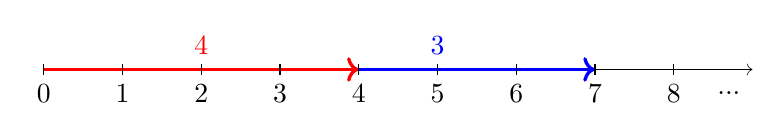
\begin{tikzpicture}
                \draw[black, very thin, ->] (0,0) -- (9,0);
                \node[] at (8.7,-0.3) {...};
                \draw[red, very thick, ->] (0,0) -- (4,0);
                    \node[red] at (2,0.3) {4};
                \draw[blue, very thick, ->] (4,0) -- (7,0);
                \node[blue] at (5,0.3) {3};
                \foreach \x/\xtext in {0/0, 1/1, 2/2, 3/3, 4/4, 5/5, 6/6, 7/7, 8/8} \draw[shift={(\x,0)}] (0pt,2pt) -- (0pt,-2pt) node[below] {$\xtext$};
            \end{tikzpicture}
            \[ 4 + 3 = 7 \]
        \end{center}
    %--- 3.1.2
    \subsubsection{Propriedades}
        \[ a+b = b+a \]
        \[ (a+b)+c = a+(b+c) \]
        \[ a+0=a \]
%------- 3.2
\subsection{Subtração}
    A subtração encontra o valor (diferença) ao reduzir um número (minuendo) por outro (subtraendo). A subtração é a operação inversa da soma, e pode ser reduzida a soma de números de sinais opostos:
    \[ a - b = a + (-b) \]
%------- 3.3
\subsection{Multiplicação}
    %--- 3.3.1
    \subsubsection{Definição}
        A multiplicação produz o resultado (produto) de uma soma finita de números iguais (coeficientes):
        \[ x \cdot y = \underbrace{x + x + ... + x}_\text{y vezes} \]
    %--- 3.3.2
    \subsubsection{Propriedades}
        \begin{multicols}{3}
            \noindent\[ a \cdot b = b \cdot a \]
            \[ (a \cdot b) \cdot c = a \cdot (b \cdot c) \]
            \[ a \cdot (b + c) = ab + ac \]
            \[ a \cdot 1 = a \]
            \[ a \cdot 0 = 0 \]
            \[ 1 \cdot (-1) = (-1) \]
            \[ (-1) \cdot (-1) = 1 \]
            \[ a \cdot \infty = \ ? \]
            \[ (a \cdot b) \in \mathbb{R} \ \forall a,b \in \mathbb{R} \]
        \end{multicols}
%------- 3.4
\subsection{Divisão}
    %--- 3.4.1
    \subsubsection{Definição}
        A divisão é a operação inversa a multiplicação, repartindo um valor (dividendo) em determinado número (quociente) de quantitativos iguais (divisor) através de sucessivas subtrações:
        \[ a \div b = q \ | \ q \cdot b = a \]
    %--- 3.4.2
    \subsubsection{Divisão Inteira}
        Quando limitada ao conjunto dos números inteiros, a divisão pode ser inexata, resultando num coeficiente para o divisor para que seu produto seja o maior número possível sem ultrapassar o dividendo, tendo como diferença o resto:
        \[ a \div b = q, r \ | \ q \cdot b + r = a \]
    %--- 3.4.3
    \subsubsection{Divisibilidade}
        Uma divisão inteira com resto zero estabelece uma relação de divisibilidade, onde o dividendo é dito como divisível pelo divisor. 
    %--- 3.4.4
    \subsubsection{Propriedades}
        \begin{multicols}{2}
            \noindent\[ a \div b \neq b \div a \]
            \[ (a \div b) \div c \neq a \div (b \div c) \]
            \[ (a+b) \div c = a \div c + b \div c \]
            \[ a \div 1 = a \]
            \[ a \div 0 = ? \]
            \[ 1 \div (-1) = (-1) \]
            \[ (-1) \div (-1) = 1 \]
        \end{multicols}
%------- 3.5
\subsection{Módulo}
    Representa o valor absoluto de um número como sua distância até a fonte na reta numérica, independentemente do sentido:
    \[ |a| = |-a| \]
%------- 3.6
\subsection{Números Primos}
    Número primo é todo aquele cujo conjunto dos divisores não inversíveis não é vazio, e todos os seus elementos são produtos dele por números inteiros inversíveis. Resumidamente é todo número inteiro cujo conjunto dos divisores naturais é composto apenas por 1 e ele mesmo.
%------- 3.7
\subsection{Fatoração}
    %--- 3.7.1
    \subsubsection{Definição}
        A fatoração é a decomposição dos coeficientes primos que iteram determinado elemento como seu produto. \eg
        \[ 2520 = 2 \cdot 2 \cdot 2 \cdot 3 \cdot 3 \cdot 5 \cdot 7 \]
    %--- 3.7.2
    \subsubsection{MDC}
        O máximo divisor comum de dois elementos pode ser encontrado ao multiplicar seus fatores primos comuns.
    %--- 3.7.3
    \subsubsection{MMC}
        O mínimo múltiplo comum de dois elementos pode ser encontrado ao dividir o produto desses números pelo seu MDC:
        \[ MMC(a,b) = \frac{a \cdot b}{MDC(a,b)} \]

        Alternativamente, o MMC pode ser encontrado ao fatora-los juntos. 
%------- 3.8
\subsection{Frações}
    %--- 3.8.1
    \subsubsection{Definição}
        É a representação de valores através da razão entre 2 números inteiros. Todo número racional possui infinitas frações equivalentes para representá-lo, que podem ser simplificadas até sua forma irredutível. \eg
        \[ \frac{256}{128} = \frac{64}{32} = \frac{4}{2} = \frac{2}{1} = 2 \]
    %--- 3.8.2
    \subsubsection{Decimais}
        Frações permitem a representação de números decimais e dízimas periódicas através de valores inteiros. \eg
        \begin{multicols}{2}
            \noindent\[ \frac{1}{5} = 0.2 \]
            \[ \frac{1}{3} = 0.\overline{333} \]
        \end{multicols}
    %--- 3.8.3
    \subsubsection{Propriedades}
        \begin{multicols}{3}
            \noindent\[ \frac{a}{c} \pm \frac{b}{c} = \frac{a \pm b}{c} \]
            \[ \frac{a}{c} \cdot \frac{b}{d} = \frac{a \cdot b}{c \cdot d} \]
            \[ \frac{a}{c} \div \frac{b}{d} = \frac{a}{c} \cdot \frac{d}{b} \]
        \end{multicols}
    %--- 3.8.4
    \subsubsection{Utilidades}
        \[ \frac{a}{c} \pm \frac{b}{d} = \frac{^a/_c \cdot MMC(c,d) \pm ^b/_d \cdot MMC(c,d)}{MMC(c,d)} \]
%------- 3.9
\subsection{Exponenciação}
    %--- 3.9.1
    \subsubsection{Definição}
        A exponenciação é definida pela multiplicação de determinado valor (base) por si próprio um determinado número de vezes (expoente). Também pode ser representada como uma função recursiva:
        \begin{multicols}{3}
            [\[ (a \in \mathbb{R}^*),(n \in \mathbb{Z}^*) \]]
            \noindent\[ a^n = a^{n-1} \cdot a \ \forall n \geq 1 \]
            \[ a^0 = 1 \]
            \[ 0^0 = ? \]
            \[ 0^n = 1 \]
            \[ \infty ^ 0 = ? \]
            \[ 1^{\infty} = ? \]
        \end{multicols}
    %--- 3.9.2
    \subsubsection{Propriedades}
        \begin{multicols}{4}
            \noindent\[ a^n \cdot a^m = a^{n+m} \]
            \[ a^n \div a^m = a^{n-m} \]
            \[ (a \cdot b)^n = a^n \cdot b^n \]
            \[ \left(\frac{a}{b} \right)^n = \frac{a^n}{b^n} \]
            \[ (a^n)^m = a^{n \cdot m} \]
            \[ a^{^n/_m} = \sqrt[m]{a^n} \]
            \[ a^{-n} = \frac{1}{a^n} \]
        \end{multicols}
    %--- 3.9.3
    \subsubsection{Utilidades}
        \begin{multicols}{2}
            \noindent\[ a^2 - b^2 = (a+b) \cdot (a-b) \]
            \[ (a \pm b)^2 = a^2 \pm 2ab + b^2 \]
            \newcolumn
            \[ (a \pm b)^3 = a^3 \pm 3a^{2}b + 3ab^2 \pm b^3 \]
            \[ (a+b)^n = \displaystyle\sum_{k=0}^{n} {\binom{n}{k} a^{n-k} b^k} \]
        \end{multicols}
%------- 3.10
\subsection{Radiciação}
    %--- 3.10.1
    \subsubsection{Definição}
        A radiciação é a operação inversa a exponenciação, onde o radicando é igual ao resultado (raiz) elevado a determinado expoente (índice):
        \[ (a \in \mathbb{R}), (n \in \mathbb{Q}^*) \]
        \[ \sqrt[n]{a} = b \ | \ b^n = a \]
    %--- 3.10.2
    \subsubsection{Propriedades}
        \begin{multicols}{3}
            \noindent\[ (\sqrt[n]{a})^m = \sqrt[n]{a^m} \]
            \[ \sqrt[n]{a^m} = \sqrt[n \cdot p]{a^{m \cdot p}} \]
            \[ \sqrt[n]{a \cdot b} = \sqrt[n]{a} \cdot \sqrt[n]{b} \]
            \[ \sqrt[n]{\left(\frac{a}{b} \right)}= \frac{\sqrt[n]{a}}{\sqrt[n]{b}} \]
            \[ \sqrt[n]{\sqrt[m]{a}} = \sqrt[n \cdot m]{a} \]
            \[ \sqrt[n]{a^m} = a^{^m/_n} \]
        \end{multicols}
    %--- 3.10.3
    \subsubsection{Utilidades}
        \begin{multicols}{2}
            \noindent\[ \sqrt{a \pm \sqrt{b}} = \sqrt{\frac{a + \sqrt{a^{2}-b}}{2}} \pm \sqrt{\frac{a - \sqrt{a^{2}-b}}{2}} \]
            \[ \sqrt{a} \approx \frac{a+b}{2 \sqrt{b}} \]
        \end{multicols}
%------- 3.11
\subsection{Logaritmação}
    %--- 3.11.1
    \subsubsection{Definição}
        A logaritmação é uma expressão análoga à exponenciação, onde seu resultado representa o expoente (logaritmo) ao qual um determinado número (base) deve ser elevado para resultar em certo valor (logaritmando):
        \begin{multicols}{2}
            [\[ (a \in \mathbb{R}^{*}-1), (b \in \mathbb{R}^*) \]]
            \noindent\[ \log_{a}b = x \ | \ a^x = b \]
            \[ \operatorname{antilog}_{a}x=b \ | \ \log_{a}b = x \]
            \[ \operatorname{colog}_{a}b = -\log_{a}b \]
            \[ \log b = \log_{10}b \]
            \[ \ln b = \log_{\mathrm{e}}b \]
            \[ \lg b = \log_{2}b \]
        \end{multicols}
    %--- 3.11.2
    \subsubsection{Propriedades}
        \begin{multicols}{2}
            \noindent\[ \log_{a}(b \cdot c) = \log_{a}b + \log_{a}c \]
            \[ \log_{a}(b \div c) = \log_{a}b - \log_{a}c \]
            \newcolumn
            \[ \log_{a}b^{\alpha} = \alpha \log_{a}b \]
            \[ \log_{a}b = \frac{\log_{c}b}{\log_{c}a} = \log_{c}b \cdot \log_{a}c \]
        \end{multicols}
    %--- 3.11.3
    \subsubsection{Utilidades}
        \begin{multicols}{2}
            \noindent\[ \log_{a}b = \frac{1}{\log_{b}a} \]
            \[ \log_{a^{\beta}}b = \frac{1}{\beta}\log_{a}b \]
        \end{multicols}
%------- 3.12
\subsection{Fatorial}
    %--- 3.12.1
    \subsubsection{Definição}
        O fatorial é uma notação para a multiplicação de um número por todos os seus antecessores inteiros:
        \[ (n \in \mathbb{N}^*) \]
        \[ n! = n \cdot (n-1) \cdot ... \cdot 2 \cdot 1 = \displaystyle\prod_{i=0}^{n-1} {n-i}  \]
        \[ 0! = 1! = 1 \]
    %--- 3.12.2
    \subsubsection{Para Números Negativos}
        \[ \Upsilon \pi o \mu o \nu \eta \]
    %--- 3.12.3
    \subsubsection{Utilidades}
        \[ (x+n)! = x! \displaystyle\prod_{k=1}^{n} {x+k} \]
%------- 3.13
\subsection{Coeficiente Binomial}
    %--- 3.13.1
    \subsubsection{Definição}
        É uma notação muito usada em combinatória, matemática diferencial e problemas com funções polinomiais:
        \[ \binom{n}{k} = \frac{n!}{k!(n-k)!} \]
    %--- 3.13.2
    \subsubsection{Relação de Stifel}
        \[ \binom{n}{k} = \binom{n-1}{k-1} + \binom{n-1}{k} \]
%------- 3.14
\subsection{Somatório}
    O somatório é uma notação para uma função recursiva de sucessivas somas:
    \[ \displaystyle\sum_{i=1}^{n} {x_i} = x_1 + x_{2} + ... + x_{n-1} + x_{n} \]
    
    \eg
    \[ \displaystyle\sum_{i=0}^{\infty} {(x!)^{-1}} = \frac{1}{0!} + \frac{1}{1!} + \frac{1}{2!} + ... \]
%------- 3.15
\subsection{Produtório}
    O produtório é uma notação para uma função recursiva de sucessivas multiplicações:
    \[ \displaystyle\prod_{i=1}^{n} {x_i} = x_1 \cdot x_{2} \cdot ... \cdot x_{n-1} \cdot x_{n} \]

    \eg
    \[ \displaystyle\sum_{i=1}^{5} {i} = 1 \cdot 2 \cdot 3 \cdot 4 \cdot 5 \]
%------- 3.16
\subsection{Ordem de Operações}
    Em expressões algébricas, existe uma ordem específica para se efetuar as operações corretamente:
    \[ \verb|parênteses| \prec \verb|expoentes| \prec \verb|multiplicações e divisões| \prec \verb|somas e subtrações| \]
    %------- ------- 4
    \section{Álgebra Elementar}
    %------- 4.1
\subsection{Sistema de Coordenadas Cartesiano}
    \[ \Upsilon \pi o \mu o \nu \eta \]
%------- 4.2
\subsection{Funções}
    %--- 4.2.1
    \subsubsection{Definição}
        Uma função é uma relação binária de dois conjuntos não vazios formando pares ordenados. A função definida A com imagem em B se da quando todo elemento de A tem exatamente um correspondente em B que cumpra sua lei de aplicação:
        \[ f:\mathcal{D} \mapsto \mathcal{CD} = \mathcal{IM} = \{ (x,y) \ | \ \forall y \in \mathcal{IM} \ \exists! x \in \mathcal{D} \ | \ f(x) = y \} \]

        Duas funções serão iguais se apresentarem iguais domínio, contradomínio, e tiverem a mesma imagem para todo elemento do domínio:
        \[ f:\mathcal{D}_f \mapsto \mathcal{CD}_f = g:\mathcal{D}_g \mapsto \mathcal{CD}_g \leftrightarrow (\mathcal{D}_f = \mathcal{D}_g) \wedge (\mathcal{CD}_f = \mathcal{CD}_g) \wedge (f(x) = g(x) \ \forall x \in \mathcal{D}) \]
    %--- 4.2.2
    \subsubsection{Classificação}
        \begin{description}
            \item[Função Sobrejetora] é aquela onde todo elemento do contradomínio tem um ou mais relacionais no domínio:
            \[ \forall y \in \mathcal{CD} \ \exists x \in \mathcal{D} \ | \ f(x) = y \]
            \item[Função Injetora] é aquela onde todo elemento do domínio tem um único ou nenhum relacional no contradomínio:
            \[ f(x_1) \neq f(x_2) \ \forall x_1, x_2 \in \mathcal{D} \ | \ x_1 \neq x_2 \]
            \item[Função Bijetora] é aquela que simultaneamente se classifica como injetora e sobrejetora, tendo assim, exatamente um relacional no contradomínio para cada elemento do domínio:
            \[ \forall x \in \mathcal{D} \ \exists! y \in \mathcal{CD} \ | \ (x,y) \in f \]
            \item[Função Simples] é aquela que não é nem injetora, nem sobrejetora. 
        \end{description}
    %--- 4.2.3
    \subsubsection{Inversão}
        Dada uma função bijetora, sua inversa é aquela cuja lei de aplicação inverte as posições de seus pares ordenados, apontando cada elemento da imagem ao seu relacional no domínio. Comumente encontrada pela inversão das operações algébricas da lei de aplicação:
        \[ f^{-1}: \mathcal{IM} \mapsto \mathcal{D} = \{(y,x) \ | \ f(x) = y\} \]
    %--- 4.2.4
    \subsubsection{Composição}
        \[ \Upsilon \pi o \mu o \nu \eta \]
    %--- 4.2.5
    \subsubsection{Categorização}
        \begin{description}
            \item[Função Identidade] é aquela que quando aplicada a qualquer elemento do domínio resulta nesse mesmo elemento. É graficamente construída como uma reta contendo as bissetrizes do $1^{\circ}$ e $3^{\circ}$ quadrantes:
            \[ f(x) = x \]
            \begin{center}
                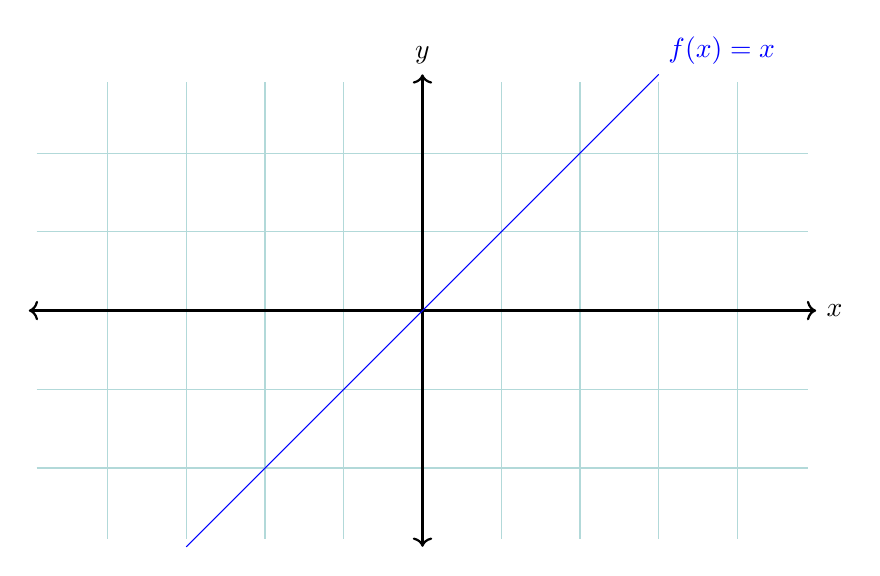
\begin{tikzpicture}
                    \draw[help lines] (-4.9,-2.9) grid (4.9,2.9);
                    \draw[black, thick, <->] (-5,0) -- (5,0) node[right]{$x$};
                    \draw[black, thick, <->] (0,-3) -- (0,3) node[above]{$y$};
                    \draw[scale=1, domain=-3:3, variable=\x, blue]  plot ({\x}, {\x}) node[above right] {$f(x) = x$};
                \end{tikzpicture}
            \end{center}
            \item[Função Linear] é aquela que quando aplicada a qualquer elemento do domínio, tem como imagem o elemento multiplicado por uma constante (coeficiente angular) diferente de 0. É construída no gráfico como uma reta que passa pela origem:
            \[ f(x) = ax \]
            \begin{center}
                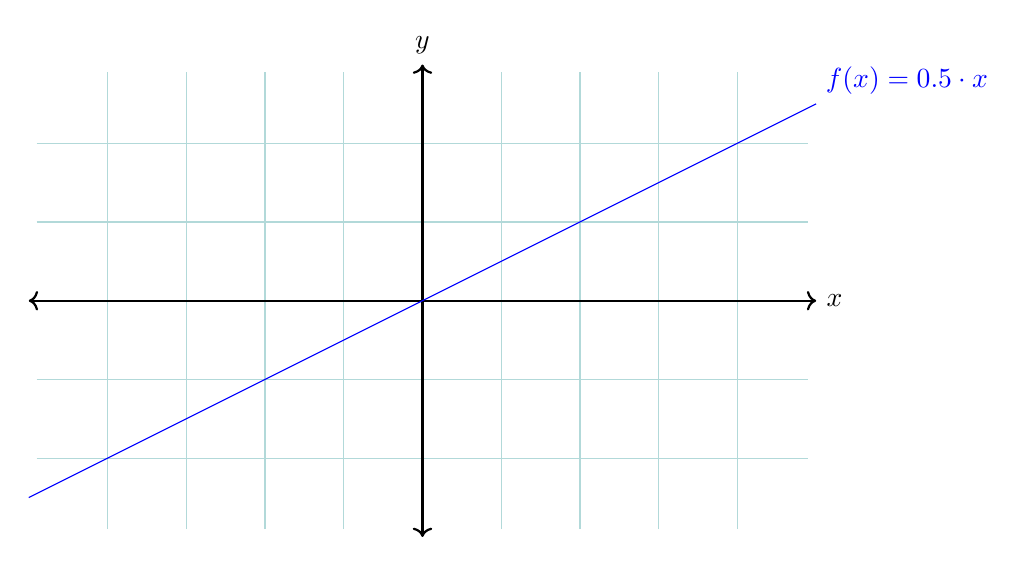
\begin{tikzpicture}
                    \draw[help lines] (-4.9,-2.9) grid (4.9,2.9);
                    \draw[black, thick, <->] (-5,0) -- (5,0) node[right]{$x$};
                    \draw[black, thick, <->] (0,-3) -- (0,3) node[above]{$y$};
                    \draw[scale=1, domain=-5:5, variable=\x, blue]  plot ({\x}, {0.5 * \x}) node[above right] {$f(x) = 0.5 \cdot x$};
                \end{tikzpicture}
            \end{center}
            \item[Função Polinomial] é aquela que tem como lei de formação uma expressão algébrica entre monômios. É classificada por grau, este que se define pelo maior expoente de sua variável:
            \[ (n \in \mathbb{N}^*), (a_n \neq 0) \]
            \[ \mathrm{P}(n) = \displaystyle\sum_{i=0}^{n} {a_{i}x^{i}} = a_{0}x^{0} + a_{1}x^{1} + ... + a_{n-1}x^{n-1} + a_{n}x^{n} \]
            \item[Função Periódica] \[ \Upsilon \pi o \mu o \nu \eta \]
            \item[Função Trigonométrica] \[ \Upsilon \pi o \mu o \nu \eta \]
            \item[Função Analítica] \[ \Upsilon \pi o \mu o \nu \eta \]
        \end{description}
    %--- 4.2.6
    \subsubsection{Graus de Funções Polinomiais}
        \begin{description}
            \item[Primeiro Grau:] chamada função afim, tem sua reta definida pelo coeficiente angular e deslocada pelo coeficiente linear:
                \[ \mathrm{P}(1) = a_{0}x^{0} + a_{1}x^{1} \]
                \[ f(x) = ax + b \]
                \begin{center}
                    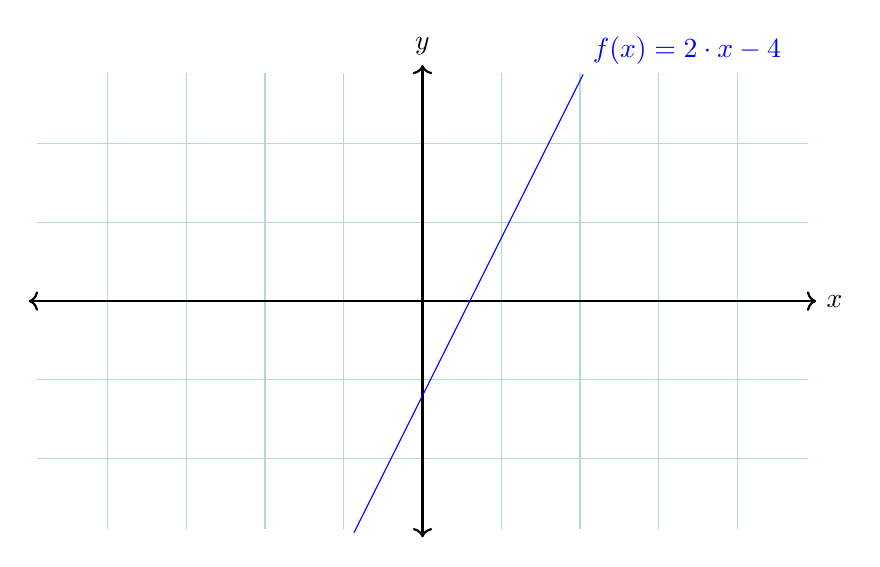
\begin{tikzpicture}
                        \draw[help lines] (-4.9,-2.9) grid (4.9,2.9);
                        \draw[black, thick, <->] (-5,0) -- (5,0) node[right]{$x$};
                        \draw[black, thick, <->] (0,-3) -- (0,3) node[above]{$y$};
                        \draw[scale=0.3, domain=-2.9:6.8, variable=\x, blue]  plot ({\x}, {2 * \x - 4}) node[above right] {$f(x) = 2 \cdot x - 4$};
                    \end{tikzpicture}
                \end{center}
                É crescente ou decrescente segundo o coeficiente angular:
                \[ (\Uparrow \ \leftrightarrow a > 0) \therefore \ (\Downarrow \ \leftrightarrow a < 0) \]
                Tem como ponto notável:
                \[ \left(\frac{-b}{a}, 0\right) \]
            \item[Segundo Grau:] chamada função quadrática, tem seu gráfico construído por uma parábola:
                \[ \mathrm{P}(2) = a_{0}x^{0} + a_{1}x^{1} + a_{2}x^{2} \]
                \[ f(x) = ax^2 + bx + c \]
                \begin{center}
                    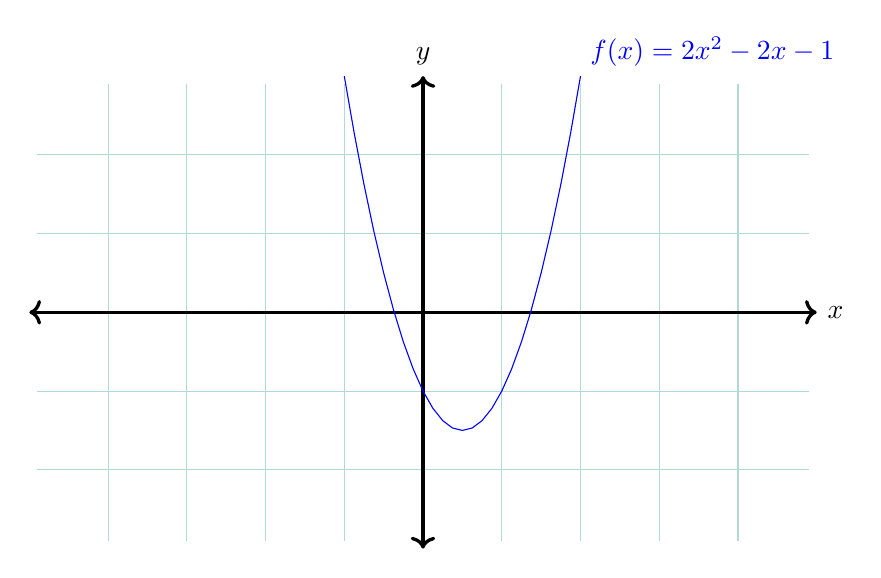
\begin{tikzpicture}
                        \draw[help lines] (-4.9,-2.9) grid (4.9,2.9);
                        \draw[black, very thick, <->] (-5,0) -- (5,0) node[right]{$x$};
                        \draw[black, very thick, <->] (0,-3) -- (0,3) node[above]{$y$};
                        \draw[scale=1, domain=-1:2, variable=\x, blue]  plot ({\x}, {2 * \x * \x - 2 * \x - 1}) node[above right] {$f(x) = 2x^2 - 2x - 1$};
                    \end{tikzpicture}
                \end{center}
                Em sua forma canônica, evidencia-se a discriminante do trinômio:
                \[ f(x) = a \left[ \left( x + \frac{b}{2a} \right)^2 - \frac{\Delta}{4a^2} \right] \]
                \[ \Delta = b^2 - 4ac \]
                O número de raízes da função é deduzível a partir da discriminante do trinômio:
                \begin{multicols}{3}
                    \noindent\[ \Delta > 0 \leftrightarrow \#R = 2 \]
                    \[ \Delta = 0 \leftrightarrow \#R = 1 \]
                    \[ \Delta < 0 \leftrightarrow \#R = 0 \]
                \end{multicols}
                A direção de abertura de sua concavidade é definida pelo primeiro coeficiente da função:
                \[ (\Uparrow \ \leftrightarrow a > 0) \therefore \ (\Downarrow \ \leftrightarrow a < 0)  \]
                Desenvolvendo sua forma canônica, encontramos formulações para facilitar a determinação das raízes da função:
                \begin{multicols}{3}
                    \noindent\[ \frac{-b \pm \sqrt{\Delta}}{2a} = \{ R_1, R_2 \} \]
                    \[ R_1 + R_2 = \frac{-b}{c} \]
                    \[ R_1 \cdot R_2 = \frac{c}{a} \]
                \end{multicols}
                Tem como pontos notáveis:
                \begin{multicols}{3}
                    \noindent\[ \left( R_1, 0 \right) \]
                    \[ P_i = \left( \frac{-b}{2a}, \frac{-\Delta}{4a} \right) \]
                    \[ \left( R_2, 0 \right) \]
                \end{multicols}
            \item[Terceiro Grau:] chamada função cúbica, tem seu gráfico construído por uma curva de dois pontos de inflexão:
                \[ \mathrm{P}(3) = a_{0}x^{0} + a_{1}x^{1} + a_{2}x^{2} + a_{3}x^{3} \]
                \[ f(x) = ax^3 + bx^2 + cx + d \]
                \begin{center}
                    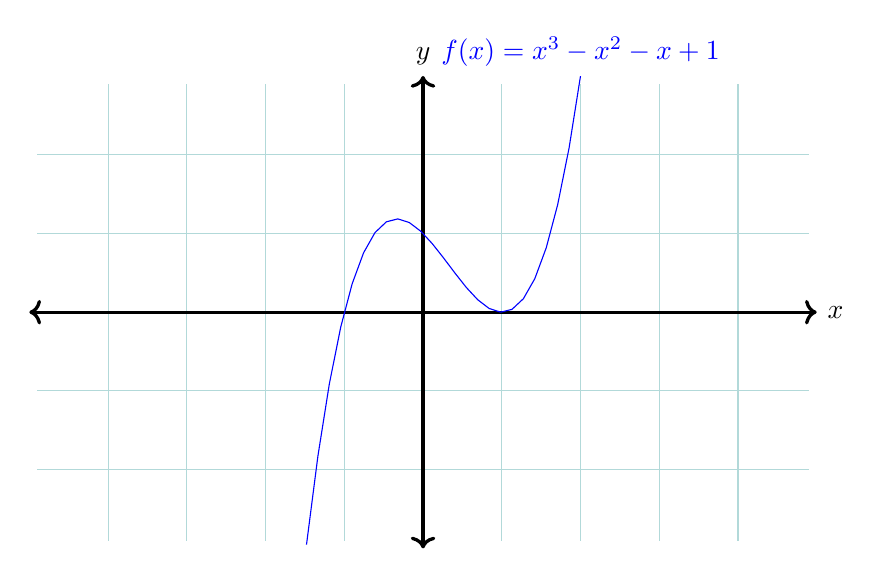
\begin{tikzpicture}
                        \draw[help lines] (-4.9,-2.9) grid (4.9,2.9);
                        \draw[black, very thick, <->] (-5,0) -- (5,0) node[right]{$x$};
                        \draw[black, very thick, <->] (0,-3) -- (0,3) node[above]{$y$};
                        \draw[scale=1, domain=-1.48:2, variable=\x, blue]  plot ({\x}, {\x * \x * \x - \x * \x - \x + 1}) node[above] {$f(x) = x^3 - x^2 - x + 1$};
                    \end{tikzpicture}
                \end{center}
                O desenvolvimento do polinômio por meio do método de Cardano-Tartaglia evidencia o discriminante da função:
                \[ \Delta = \left(\frac{ c + \frac{2a^3 - 9ab}{27}}{2}\right)^2 + \left(\frac{ b - \frac{a^2}{3}}{3}\right)^3 \]
                O número de raízes da função é deduzível a partir da discriminante da função:
                \[ \Delta > 0 \leftrightarrow \{ R_i, R_j, R_k \} \ | \ (R_i \in \mathbb{R}), (R_j, R_k \in \mathbb{C}) \]
                \[ \Delta = 0 \leftrightarrow \{ R_i, R_j, R_k \} \ | \ (R_i, R_j, R_k \in \mathbb{R}), (R_j = R_k) \]
                \[ \Delta < 0 \leftrightarrow \{ R_i, R_j, R_k \} \ | \ (R_i, R_j, R_k \in \mathbb{R}), (R_i \neq R_j \neq R_k) \]
                Usando a solução do método de Cardano-Tartaglia é possível encontrar as raízes da função:
                \[ p = \frac{c}{a} - \frac{b^2}{3a^2} \hphantom{---} q = \frac{d}{a} - \frac{bc}{3a^2} + \frac{2b^3}{27a^3}\]
                \[ R_1 = \frac{-b}{3a} + \sqrt[3]{\frac{-q}{2} + \sqrt{\left(\frac{q}{2} \right)^2 + \left(\frac{p}{3} \right)^3}} + \sqrt[3]{\frac{-q}{2} - \sqrt{{\left(\frac{q}{2} \right)^2 + \left(\frac{p}{3} \right)^3}}} \]
                \[ R_2 = \frac{-b}{3a} + \left( \frac{-1}{2} + \frac{\mathrm{i\sqrt{3}}}{2} \right) \sqrt[3]{\frac{-q}{2} + \sqrt{{\left(\frac{q}{2} \right)^2 + \left(\frac{p}{3} \right)^3}}} + \left( \frac{-1}{2} - \frac{\mathrm{i\sqrt{3}}}{2} \right) \sqrt[3]{\frac{-q}{2} - \sqrt{{\left(\frac{q}{2} \right)^2 + \left(\frac{p}{3} \right)^3}}} \]
                \[ R_2 = \frac{-b}{3a} + \left( \frac{-1}{2} + \frac{\mathrm{i\sqrt{3}}}{2} \right) \sqrt[3]{\frac{-q}{2} - \sqrt{{\left(\frac{q}{2} \right)^2 + \left(\frac{p}{3} \right)^3}}} + \left( \frac{-1}{2} - \frac{\mathrm{i\sqrt{3}}}{2} \right) \sqrt[3]{\frac{-q}{2} + \sqrt{{\left(\frac{q}{2} \right)^2 + \left(\frac{p}{3} \right)^3}}} \]
                Para além deste método, há outras ferramentas para facilitar a determinação das raízes:
                \begin{itemize}
                    \item[$\implies$] Relações de Girard:
                    \[ R_1 + R_2 + R_3 = \frac{-b}{a} \hphantom{---} R_1 \cdot R_2 \cdot R_3 = \frac{-d}{a}\]
                    \[ R_1 \cdot R_2 + R_1 \cdot R_3 + R_2 \cdot R_3 = \frac{c}{a} \]
                    \item[$\implies$] Fatoração da Equação: \[ \Upsilon \pi o \mu o \nu \eta \]
                    \item[$\implies$] Listagem de Razão Entre Fatores: \[ \Upsilon \pi o \mu o \nu \eta \]
                \end{itemize}
        \end{description}
    %--- 4.2.7
    \subsection{Interpolação Polinomial}
        \[ \Upsilon \pi o \mu o \nu \eta \]
    %--- 4.2.8
    \subsection{Divisão de Polinômios}
        \[ \Upsilon \pi o \mu o \nu \eta \]
    %--- 4.2.9
    \subsection{Fatoração de Funções Polinomiais}
        \[ \Upsilon \pi o \mu o \nu \eta \]
%------- 4.3
\subsection{Equações}
    %--- 4.3.
    \subsubsection{Equação Quadrática}
        \[ \Upsilon \pi o \mu o \nu \eta \]
    %--- 4.3.
    \subsubsection{Equação Biquadrática}
        \[ \Upsilon \pi o \mu o \nu \eta \]
    %--- 4.3.
    \subsubsection{Equação Cúbica}
        \[ \Upsilon \pi o \mu o \nu \eta \]
    %--- 4.3.
    \subsubsection{Equação Circular}
        \[ \Upsilon \pi o \mu o \nu \eta \]
%------- 4.4
\subsection{Inequações}
    %--- 4.4.1
    \subsubsection{Definição}
        Inequações são expressões algébricas de desigualdade, formando-se por sentenças matemáticas que expressam uma relação de não-equivalência entre funções:
        \[ f \star g \]
        O domínio de validade de uma inequação é a interseção dos domínios das funções, e a sua solução é dada pelo conjunto de todos os elementos do domínio de validade que cumpram a sentença de desigualdade:
        \[\mathcal{D}_{f \star g} = \mathcal{D}_f \cap \mathcal{D}_g \hphantom{---}  S_{f \star g} = \{ x \in \mathcal{D}_{f \star g} \ | \ f(x) \star g(x) \} \]
    %--- 4.4.2
    \subsubsection{Princípios de Equivalência}
        Inequações são ditas equivalentes quando possuem iguais conjuntos solução, e na resolução de uma inequação, busca-se a forma mais simples da sentença de desigualdade, tendo como referência os princípios de equivalência:
        \[ (f: \mathcal{D}_f \mapsto \mathcal{CD}_f), (g: \mathcal{D}_g \mapsto \mathcal{CD}_g), (h: \mathcal{D}_{f \star g} \mapsto \mathcal{CD}_{f \star g}) \]
        \begin{description}
            \item[P-1:] em uma inequação, podemos transpor um termo de um membro para outro trocando o sinal do termo considerado:
            \[ f + h \star g \equiv f \star g - h \]
            \[ f \star g \equiv f + h \star g + h \]
            \item[P-2:] em uma inequação, podemos multiplicar os dois membros pela mesma expressão, mantendo ou invertendo o sentido da desigualdade, conforme essa expressão seja positiva ou negativa, respectivamente:
            \[ f \ \overrightarrow{\star} \ g  \equiv \begin{dcases} f(x) \cdot h(x) \overrightarrow{\star} g(x) \cdot h(x) \leftrightarrow h(x) > 0 \\ f(x) \cdot h(x) \overleftarrow{\star} g(x) \cdot h(x) \leftrightarrow h(x) < 0 \end{dcases} \]
        \end{description}
    %--- 4.4.3
    \subsubsection{Simultâneas}
        Inequações simultâneas são a conjunção de 2 inequações alinhadas, e portanto, seu conjunto solução será a interseção do conjunto solução das inequações quando decompostas e resolvidas individualmente:
        \[ f \star g \star h \equiv \begin{dcases} f \star g \\ g \star h \end{dcases} \ \rightarrow \ S_{f \star g \star h} = S_{f \star g} \cap S_{g \star h} \]
%------- 4.5
\subsection{Sequências}
    %--- 4.5.1
    \subsubsection{Definição}
        Uma sequência é uma função onde o domínio é limitado ao conjunto dos números naturais não-nulos, assim indexando o contradomínio através da lei de aplicação e formando a imagem como uma lista ordenada. Sequências podem ser finitas ou infinitas:
        \begin{multicols}{2}
            \noindent\[ f:\mathbb{N}^i \mapsto \mathbb{R} = \{ (i, t_i) \forall i \in \mathbb{N}^i \} \]
            \[ f:\mathbb{N} \mapsto \mathbb{R} = \{ (i, t_i) \forall i \in \mathbb{N} \} \]
        \end{multicols}
    %--- 4.5.2
    \subsubsection{Lei de Formação}
        A lei de formação de uma sequência é sua lei de aplicação, e pode ser apresentada de 3 distintas formas:
        \begin{description}
            \item[Fórmula de Recorrência:] define-se o primeiro termo e a regra para encontrar seus subsequentes. \eg
            \[ f = \begin{dcases} t_1 = 1 \\ t_i = t_{i-1} + t_{i-2} \end{dcases} \forall i \in \mathbb{N} \ = \ \{1,1,2,3,5,8,13,21,...\} \]
            \item[Fórmula Geral:] a lei de aplicação expressa cada termo através de seu índice. \eg
            \[ b = \{ (i,t_i) \ | \ t_i = 2^i \ \forall i \in \mathbb{N} \} = \{2,4,8,16,32,64,128,256,...\} \]
            \item[Propriedade dos Termos:] é descrita uma propriedade que os termos devem cumprir. \eg
            \[ p = \text{todos os números primos em ordem crescente} = \{2,3,5,7,11,13,...\} \]
        \end{description}
    %--- 4.5.3
    \subsubsection{Progressão Aritmética}
        \begin{description}
            \item[Definição:] é toda sequência definida por fórmula de recorrência onde todo termo é igual ao seu antecedente somado a uma constante (razão), podendo ser classificada como crescente, decrescente ou constante em função dessa constante:
            \[ P.A. = \begin{dcases} t_1 = n \\ t_i = t_{i-1} + r \end{dcases} \ \rightarrow \ t_i = t_1 + r(i-1) \]
            \item[Interpolação Aritmética:] é inserir meios aritméticos entre dois extremos definidos, onde a razão será encontrada a partir do número de elementos interpolados:
            \[ r = \frac{t_i - t_1}{i - 1} \]
            \item[Soma dos Termos:] fórmula geral para a soma dos termos de uma progressão aritmética:
            \[ S_i = \frac{i(t_1 + t_i)}{2} \ = \ i \cdot t_1 + r \frac{i(i-1)}{2} \]
        \end{description}
    %--- 4.5.4
    \subsubsection{Progressão Geométrica}
        \begin{description}
            \item[Definição:] é toda sequência definida por fórmula de recorrência, onde todo termo é igual ao seu antecedente multiplicado por uma constante (razão), podendo ser classificada como crescente, constante, decrescente, alternante (quando os termos alternam os sinais) ou estacionária (quando a razão é zero):
            \[ P.G. = \begin{dcases} t_1 = n \\ t_i = t_{i-1} \cdot r \end{dcases} \ \rightarrow \ t_i = t_1 \cdot r^{i-1} \]
            \item[Interpolação Geométrica:] é inserir meios geométricos entre dois extremos definidos, onde a razão será encontrada a partir do número de elementos interpolados:
            \[ r = \sqrt[i-1]{\frac{t_i}{t_1}} \]
            \item[Soma dos Termos:] fórmula geral para a soma dos termos de uma progressão geométrica:
            \[ S_i = t_1 \frac{r^i -1}{r - 1} \ = \ t_i \frac{r-t_1}{r-1} \]
            \item[Produto dos Termos:] fórmula geral para o produto dos termos de uma progressão geométrica:
            \[ P_i = t_1^i \cdot r^{\frac{i(i-1)}{2}} = (t_1 \cdot t_i)^{\frac{i}{2}} \]
        \end{description}
    %------- ------- 5
    \section{Álgebra Linear}
    %------- 5.1
\subsection{Matrizes}
    %--- 5.1.1
    \subsubsection{Definição}
        Matriz é toda tabela formada por números reais, caracterizada pelo número de linhas e colunas, respectivamente, contadas de cima para baixo e da esquerda para direita:
        \[ (x, y, i, j \in \mathbb{N}) \]
        \[ M_{y \times x} = \begin{bmatrix} a_{1 \; 1} & & a_{1 \; x} \\ & \cdots & \\ a_{y \; 1} &  & a_{y \; x} \end{bmatrix} \ | \ a_{i \; j} \in \mathbb{R} \ \forall i \in \mathbb{N}^y \wedge  \forall j \in \mathbb{N}^x \]
    %--- 5.1.2
    \subsubsection{Classificações}
        \begin{description}
            \item[Matriz Nula:] é toda matriz onde todos os seus elementos são iguais a zero:
            \[ M_{y \times x} = \{a_{i \; j} = 0 \ | \ \forall i \in \mathbb{N}^y \wedge  \forall j \in \mathbb{N}^x \} \]
            \item[Matriz Linha:] é toda matriz que composta por uma única linha. \eg
            \[ M_{1 \times x} = \begin{bmatrix} a_{1 \; 1} & \cdots & a_{1 \; x} \end{bmatrix} \]
            \item[Matriz Coluna:] é toda matriz que composta por uma única coluna. \eg
            \[ M_{y \times 1} = \begin{bmatrix} a_{1 \; 1} \\ \vdots \\ a_{y \; 1} \end{bmatrix} \]
            \item[Matriz Quadrada:] é toda matriz com o mesmo número de linhas e colunas, onde este número é apontado como o seu grau. \eg
            \[ M_{n \times n} = \begin{bmatrix} a_{1 \; 1} & & a_{1 \; n} \\ & \cdots & \\ a_{n \; 1} &  & a_{n \; n} \end{bmatrix} \]
            Na matriz quadrada denota-se a importância de suas duas diagonais, a principal e secundária, respectivamente:
            \[ a_{i \; j} \in M_{n \times n} \ | \ i = j \hphantom{---} a_{i \; j} \in M_{n \times n} \ | \ i + j = n + 1 \]
            \item[Matriz Diagonal:] é toda matriz quadrada onde os elementos não pertencentes a diagonal principal são nulos. \eg
            \[ \begin{bmatrix} a_{1 \; 1} & 0 & 0 \\ 0 & a_{2 \; 2} & 0 \\ 0 & 0 & a_{3 \; 3} \end{bmatrix} \]
            \item[Matriz Identidade:] é toda matriz quadrada onde os elementos da diagonal principal são iguais a 1, enquanto todos os outros elementos são nulos. \eg
            \[ I_3 = \begin{bmatrix} 1 & 0 & 0 \\ 0 & 1 & 0 \\ 0 & 0 & 1 \end{bmatrix} \]
            \item[Matriz Triangular:] toda matriz quadrada onde os elementos acima ou abaixo da diagonal principal são nulos:
            \[ a_{i \; j} = 0 \ \forall i < j \vee j > i \]
        \end{description}
    %--- 5.1.3
    \subsubsection{Adição}
        A soma de duas matrizes (necessariamente de mesma dimensão) é feita pela soma de seus respectivos termos:
        \[ A_{y \times x} + B_{y \times x} = C_{y \times x} \ | \ c_{i \; j} = b_{i \; j} + a_{i \; j} \]
    %--- 5.1.4
    \subsubsection{Multiplicação}
        \begin{description}
            \item[Por um Coeficiente:] a multiplicação de uma matriz por um número é feita multiplicando cada um de seus elementos pelo coeficiente: 
            \[ A_{y \times x} \cdot k = B_{y \times x} \ | \ b_{i \; j} = k \cdot a_{i \; j} \]
            \item[Por Outra Matrix:] a multiplicação de duas matrizes (necessariamente tendo o número de colunas da primeira igual ao número de linhas da segunda) resulta numa matriz contendo a somatório do produto dos elementos ordenados em linha por coluna:
            \[ A_{m \times n} \cdot B_{n \times p} = C_{m \times p} \ | \ c_{i \; j} = \displaystyle\sum_{k=1}^{n} {a_{i \; k} \cdot b_{k \; j}} \]
            Nota-se que: $ M_{y \times x} \cdot I_y = I_y \cdot M_{y \times x} = M_{y \times x} $
        \end{description}
    %--- 5.1.5
    \subsubsection{Transposição}
        A transposição de uma matriz é seu espelhamento, invertendo a indexação de linhas e colunas de seus elementos:
        \[ M_{y \times x} = a_{i \; j} \xrightarrow{\text{transposição}} M_{x \times y}^t = a_{j \times i} \]
        Frente ao processo de transposição matricial, surgem duas classificações:
        \begin{description}
            \item[Matriz Simétrica:] é toda matriz quadrada equivalente a sua transposição.
            \item[Matriz Antissimétrica:] é toda matriz quadrada cuja qual, quando transposta, resulta na sua matriz oposta.
        \end{description}
        %--- 5.1.6
        \subsubsection{Inversão}
        Uma matriz quadrada é dita inversível quando existe uma inversa que multiplicada por ela resulta numa matriz identidade de mesma ordem:
        \[ M_{n \times n} \cdot M_{n \times n}^{-1} = M_{n \times n}^{-1} \cdot M_{n \times n} = I_n \]
%------- 5.2
\subsection{Determinantes}
    %--- 5.2.1
    \subsubsection{Definição}
        O determinante é uma função matricial que associa matrizes quadradas a um escalar que a define e mede sua transformação no espaço vetorial, possuindo inúmeras aplicações em campos diversos da matemática e física. Para matrizes de primeira e segunda ordem, o determinante é encontrado da seguinte forma:
        \[ \det{M_{1 \times 1}} = \begin{vmatrix} a_{1 \; 1} \end{vmatrix} = a_{1 \; 1} \]
        \begin{center}
            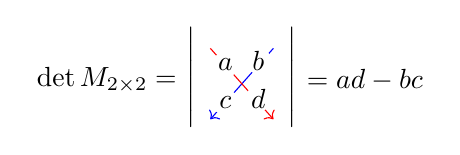
\begin{tikzpicture}
                \begin{pgfonlayer}{fg}
                    \matrix (M) [matrix of math nodes, left delimiter  = |, right delimiter = |] at (0,0) { a & b  \\ c & d \\ } node [left=20pt] {$ \det{M_{2 \times 2}} = $} node[right=20pt] {$ = ad - bc $};
                \end{pgfonlayer}
                \begin{pgfonlayer}{main}
                    \node[circle, fill=white] at (M-1-1) {};
                    \node[circle, fill=white] at (M-1-2) {};
                    \node[circle, fill=white] at (M-2-1) {};
                    \node[circle, fill=white] at (M-2-2) {};
                \end{pgfonlayer}
                \begin{pgfonlayer}{bg}
                    \draw[blue, ->] (0.4,0.4) -- (-0.4,-0.5);
                    \draw[red, ->] (-0.4,0.4) -- (0.4,-0.5);
                \end{pgfonlayer}
            \end{tikzpicture}
        \end{center}
    %--- 5.2.2
    \subsubsection{Regra de Sarrus}
        Para matrizes de terceira ordem, usamos a seguinte regra:
        \begin{center}
            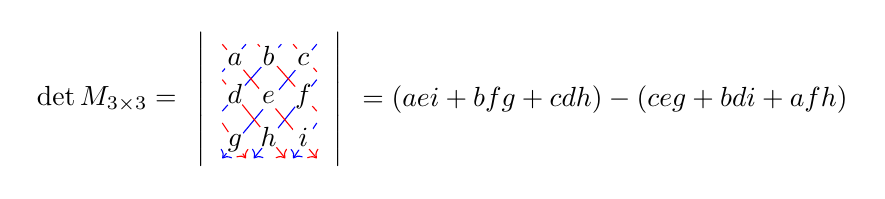
\begin{tikzpicture}
                \begin{pgfonlayer}{fg}
                    \matrix (M) [matrix of math nodes, left delimiter  = |, right delimiter = |] at (0,0) { a & b & c \\ d & e & f \\ g & h & i \\ } node [left=30pt] {$ \det{M_{3 \times 3}} =  $} node[right=30pt] {$ = (aei + bfg + cdh) - (ceg + bdi + afh) $};
                \end{pgfonlayer}
                \begin{pgfonlayer}{main}
                    \node[circle, fill=white] at (M-1-1) {};
                    \node[circle, fill=white] at (M-1-2) {};
                    \node[circle, fill=white] at (M-1-3) {};

                    \node[circle, fill=white] at (M-2-1) {};
                    \node[circle, fill=white] at (M-2-2) {};
                    \node[circle, fill=white] at (M-2-3) {};

                    \node[circle, fill=white] at (M-3-1) {};
                    \node[circle, fill=white] at (M-3-2) {};
                    \node[circle, fill=white] at (M-3-3) {};
                \end{pgfonlayer}
                \begin{pgfonlayer}{bg}
                    \draw[blue, ->] (0.6,0.7) -- (-0.6,-0.75);
                    \draw[blue, -] (0.15,0.7) -- (-0.6,-0.15);
                    \draw[blue, -] (-0.3,0.7) -- (-0.6,0.35);
                    \draw[blue, ->] (0.6,0.25) -- (-0.2,-0.75);
                    \draw[blue, ->] (0.6,-0.3) -- (0.3,-0.75);

                    \draw[red, ->] (-0.6,0.7) -- (0.6,-0.75);
                    \draw[red, -] (-0.15,0.7) -- (0.6,-0.15);
                    \draw[red, -] (0.3,0.7) -- (0.6,0.35);
                    \draw[red, ->] (-0.6,0.25) -- (0.2,-0.75);
                    \draw[red, ->] (-0.6,-0.3) -- (-0.3,-0.75);
                \end{pgfonlayer}
            \end{tikzpicture}
        \end{center}
    %--- 5.2.3
    \subsubsection{Menor Complementar}
        Para uma matriz de ordem maior que 2, o complementar algébrico de um elemento é o determinante que se obtém ao suprimir a linha e coluna desse elemento. \eg
        \[ M_{3 \times 3} = \begin{vmatrix} a & b & c \\ d & e & f \\ g & h & i \\ \end{vmatrix} : D_{1 \; 1} =  \begin{vmatrix} e & f\\ h & i\end{vmatrix}; D_{2 \; 2} =  \begin{vmatrix} a & c\\ g & i \end{vmatrix}; D_{3 \; 3} =  \begin{vmatrix} a & b \\ d & e \end{vmatrix} \]
        %--- 5.2.4
        \subsubsection{Complemento Algébrico}
        Para uma matriz de ordem maior que 2, o complemento algébrico (cofator) de um elemento é dado por:
        \[ A_{i \; j} = (-1)^{i + j} \cdot D_{i \; j} \]
    %--- 5.2.5
    \subsubsection{Determinante por Recorrência}
        A definição da determinante por recorrência (caso geral) é dada pela soma dos produtos dos elementos da primeira coluna por seus complementos algébricos:
        \[ \det{M_{n \times n}} = \displaystyle\sum_{i=i}^{n} {a_{i \; 1} \cdot A_{i \; 1} } \]
    %--- 5.2.6
    \subsubsection{Teorema de Laplace}
        O teorema de Laplace diz que o determinante de uma matriz de ordem maior que 2 é a soma dos produtos dos elementos de uma fila qualquer por seus respectivos cofatores, assim a definição do determinante por recorrência não precisa ser aplicado necessariamente à primeira coluna, mas a qualquer linha ou coluna de uma matriz.
    %--- 5.2.7
    \subsubsection{Combinação Linear}
        Define-se pelo conjunto das somas dos produtos dos elementos de determinadas filas por determinadas constantes, ordenadamente:
        \[ M_{n \times n} = [a_{i \; j}] \hphantom{---} s=\{filas \: paralelas \} \hphantom{---} p = \# s \hphantom{---} c = \{ c_1,...,c_p \}\]
        \[ \alpha = \{ \alpha_1, ..., \alpha_n \} \ | \ \alpha_{\sigma} =  \begin{dcases}  \displaystyle\sum_{k=1}^{p} {a_{s_k \; \sigma} \cdot c_k} \because s = \{linhas\} \\ \displaystyle\sum_{k=1}^{p} {a_{\sigma \; s_k} \cdot c_k} \because s = \{colunas\} \end{dcases} \]

        \eg
        \[ M_{3 \times 3} = [a_{i \; j}] \]
        \[ s_{x} = \{ 2,3 \}, c=\{q,r\} \rightarrow \alpha = \begin{dcases} \alpha_1 = a_{2 \; 1} \cdot q + a_{3 \; 1} \cdot r \\ \alpha_2 = a_{2 \; 2} \cdot q + a_{3 \; 2} \cdot r \\ \alpha_3 = a_{2 \; 3} \cdot q + a_{3 \; 3} \cdot r \end{dcases} \]
        \[ s_{y} = \{1,2,3\}, c=\{q,r,s\} \rightarrow \alpha = \begin{dcases} \alpha_{1} = a_{1 \; 1} \cdot q + a_{1 \; 2} \cdot r + a_{1 \; 3} \cdot s \\ \alpha_{2} = a_{2 \; 1} \cdot q + a_{2 \; 2} \cdot r + a_{2 \; 3} \cdot s \\ \alpha_{3} = a_{3 \; 1} \cdot q + a_{3 \; 2} \cdot r + a_{3 \; 3} \cdot s \end{dcases} \]
    %--- 5.2.8
    \subsubsection{Propriedades}
        \begin{description}
            \item[P-1:] o determinante de uma matriz é igual ao de sua transposta:
            \[ \det{M} = \det{M^t} \]
            \item[P-2:] se os elementos de uma fila qualquer de uma matriz forem todos nulos, então o determinante dessa matriz é zero.
            \item[P-3:] se multiplicada uma fila qualquer de uma matriz por uma constante, o valor do determinante dessa matriz também é multiplicado pela mesma constante. \eg
            \[ k \cdot \begin{vmatrix} a & b & c \\ d & e & f \\ g & h & i \end{vmatrix} = \begin{vmatrix} a & kb & c \\ d & ke & f \\ g & kh & i \end{vmatrix} \]
            \[ \det{(k \cdot M_{n \; n})} = k^n \cdot \det{M_{n \; n}} \]
            \item[P-4:] se invertidas as posições de 2 filas paralelas de uma matriz, o determinante da nova matriz formada será o oposto do determinante da primeira. \eg
            \[ \begin{vmatrix} a & b & c \\ d & e & f \\ g & h & i \end{vmatrix} = -1 \cdot \begin{vmatrix} b & a & c \\ e & d & f \\ h & g & i \end{vmatrix} \]
            \item[P-5:] se uma matriz tem 2 filas paralelas idênticas, por consequência da P-4 o determinante será 0.
            \item[P-6:] a soma dos produtos dos elementos de uma fila qualquer pelos cofatores de uma fila paralela resulta em 0:
            \[ A_{n \times n} = [a_{i \; j}] \hphantom{---} (p \in \mathbb{N}^n - i) \hphantom{---} (q \in \mathbb{N}^n - j) \]
            \[ \sum_{i=1}^{n} {a_{i \; j} \cdot A_{p \; j}} = \sum_{j=1}^{n} {a_{i \; j} \cdot A_{i \; q}} = 0 \]
            \item[P-7:] se duas filas paralelas de uma matriz forem formadas por elementos respectivamente proporcionais, então seu determinante será 0:
            \[ (A_{n \times n} = [a_{i \; j}]) \hphantom{---} (p \in \mathbb{N}^n - i) \hphantom{---} (q \in \mathbb{N}^n - i) \hphantom{---} (k = \{ \alpha \in \mathbb{R} \ | \ \#k = n \}) \]
            \[ \begin{matrix} a_{i \; j} = a_{p \; j} \cdot k_j \\ a_{i \; j} = a_{i \; q} \cdot k_i \end{matrix} \bigg{\}} \rightarrow \det{A} = 0 \]
            \item[P-8:] caso tomada uma matriz e decompostos os elementos de uma fila qualquer em uma soma de dois elementos, o determinante dessa matriz será a soma dos determinantes das matrizes formadas pela substituição dessa fila pelas parcelas da soma. \eg
            \[ \begin{vmatrix} a & (b_1 + b_2) & c \\ d & (e_1 + e_2) & f \\ g & (h_1 + h_2) & i \end{vmatrix} = \begin{vmatrix} a & b_1 & c \\ d & e_1 & f \\ g & h_1 & i \end{vmatrix} + \begin{vmatrix} a & b_2 & c \\ d & e_2 & f \\ g & h_2 & i \end{vmatrix} \]
            \item[P-9:] se uma matriz quadrada tiver uma de suas filas como a combinação linear de suas outras filas, então o determinante dessa matriz é 0. \eg
            \[ \begin{vmatrix} 0 & 1 & 2 \\ 2 & 3 & 8 \\ 4 & 5 & 14 \end{vmatrix} = 0 \because \{a_{1 \; 3}, a_{2 \; 3}, a_{3 \; 3}\} = \{\alpha_1, \alpha_2, \alpha_3\} \ | \ s_y = \{1,2\}, c=\{1,2\} \]
            \item[P-10:] se uma fila qualquer de uma matriz quadrada for multiplicada por uma constante e somada a outra fila paralela, o determinante se mantém inalterado. \eg
            \[ \begin{vmatrix} a & b & c \\ d & e & f \\ g & h & i \end{vmatrix} = \begin{vmatrix} a & (b + ka) & c \\ d & (e + kd) & f \\ g & (h + kg) & i \end{vmatrix} \]
            \item[P-11:] o determinante de uma matriz triangular é igual ao produto dos elementos da diagonal principal. \eg
            \[ \begin{vmatrix} a & 0 & 0 \\ d & e & 0 \\ g & h & i \end{vmatrix} = a \cdot e \cdot i \]
            \item[P-12:] dadas duas matrizes quadradas de mesma ordem, o determinante do produto das matrizes é igual ao produto dos determinantes das matrizes:
            \[ A_{n \times n}, B_{n \times n} \leftarrow \det{(A \cdot B)} = \det{A} \cdot \det{B} \]
        \end{description}
    %--- 5.2.9
    \subsubsection{Redução da Ordem}
        Usando o teorema de Jacobi (P-10) e o teorema de Laplace, é possível reduzir a ordem de um determinante, desde que o primeiro elemento da primeira coluna da matriz tenha valor 1:
        \[ A_{n \times n} = \begin{bmatrix} 1 & a_{1 \; 2} & \cdots & a_{1 \; n} \\ a_{2 \; 1} & a_{2 \; 2} & \cdots & a_{2 \; n} \\ \vdots & \vdots & \ddots & \vdots \\ a_{n \; 1} & a_{n \; 2} & \cdots  & a_{n \; n} \end{bmatrix} \]
        
        Soma-se a primeira coluna a cada uma das restantes, multiplicadas pelo oposto de seu respectivo primeiro elemento:
        \[ B_{n \times n} = [b_{i \; j}] \ | \ \begin{dcases} b_{1 \; 1} = 1 \\ b_{i \; j} = a_{i \; j} + a_{i \; 1} \cdot (-a_{1 \; j}) \forall i \in \mathbb{N}^n, j \in \mathbb{N}^n -1 \end{dcases} \]
        \[ B = \begin{bmatrix} 1 & (a_{1 \; 2} -1 a_{1 \; 2}) & \cdots & (a_{1 \; n} -1 a_{1 \; n}) \\ a_{2 \; 1} & (a_{2 \; 2} - a_{2 \; 1} \cdot a_{1 \; 2}) & \cdots & (a_{2 \; n} - a_{2 \; 1} \cdot a_{1 \; n}) \\ \vdots & \vdots & \ddots & \vdots \\ a_{n \; 1} & (a_{n \; 2} - a_{n \; 1} \cdot a_{1 \; 2}) & \cdots  & (a_{n \; n} - a_{n \; 1} \cdot a_{1 \; n}) \end{bmatrix} = \begin{bmatrix} 1 & 0 & \cdots & 0 \\ b_{2 \; 1} & b_{2 \; 2} & \cdots & b_{2 \; n} \\ \vdots & \vdots & \ddots & \vdots \\ b_{n \; 1} & b_{n \; 2} & \cdots  & b_{n \; n} \end{bmatrix} \]
        
        Por fim, aplicando o teorema de Laplace:
        \[ \det{A} = \det{B} = \begin{vmatrix} b_{2 \; 2} & \cdots & b_{2 \; n} \\ \vdots & \ddots & \vdots \\ b_{2 \; n} & \cdots & b_{n \; n} \end{vmatrix} \]
    %--- 5.2.10
    \subsubsection{Regra de Chió}
        Simplificando o processo de redução de ordem de uma matriz, a regra de Chió diz que, sendo o primeiro elemento de uma matriz quadrada igual a 1, encontra-se uma matriz de ordem imediatamente menor com igual determinante suprimindo a primeira linha e coluna da matriz inicial, e em seguida subtraindo cada elemento do produto dos extremos de sua posição:
        \[ A_{n \times n} = [a_{i \; j}] \ | \ a_{1 \; 1} = 1 \hphantom{---} B_{n-1 \times n-1} = [b_{i \; j}] \ | \ b_{i \; j} = a_{(i+1) \; (j+1)} - a_{(i+1) \; 1} \cdot a_{1 \; (j+1)} \]
        \[ \det{A} = \det{B} \]
        
        \eg
        \[ \begin{vmatrix} 1 & b & c \\ d & e & f \\ g & h & i \end{vmatrix} = \begin{vmatrix} (e - bd) & (f-cd) \\ (h -bg) & (i -cg) \end{vmatrix} \]
    %--- 5.2.11
    \subsubsection{Matriz de Vandermonde}
        Também conhecida como matriz das potências, matriz de Vandermonde é toda aquela que se define por filas paralelas de progressões geométrica com seus primeiros elementos iguais a um, e segundos elementos chamados característicos. Essas matrizes têm seu determinante encontrado pelo prodututório do arranjo das diferenças entre os elementos característicos:
        \[ V_{n \times n} = [v_{i \; j}] \ | \ \begin{dcases} a_{i \; j} = a_{2 \; j}^{i-1} \\ a_{i \; j} = a_{i \; 2}^{j-1} \end{dcases} \]
        \[ \det{V_x} = \displaystyle\prod_{1 \leq p < q \leq n} {v_{2 \; q} - v_{2 \; p}} \hphantom{---} \det{V_y} = \displaystyle\prod_{1 \leq p < q \leq n} {v_{q \; 2} - v_{p \; 2}} \]

        \eg
        \[ \begin{vmatrix} a^0 & b^0 & c^0 \\ a^1 & b^1 & c^1 \\ a^2 & b^2 & c^2 \end{vmatrix} = (b^1 - a^1) \cdot (c^1 - a^1) \cdot (c^1 - b^1) \]
    %--- 5.2.12
    \subsubsection{Matriz Adjunta}
        Chama-se matriz adjunta aquela obtida pela substituição dos elementos da matriz inicial por seus respectivos complementos algébricos, seguida da transposição da matriz:
        \[ M_{n \times n} = [a_{i \; j}] \hphantom{---} \overline{M}_{n \times n} = [A_{j \; i}] \]
        
        Com a aplicação dos teoremas de Laplace e Cauchy, encontra-se uma propriedade sobre o determinante da matriz inicial, e por consequência dessa, é possível calcular a sua inversa:
        \[ M \cdot \overline{M} = \overline{M} \cdot M = \det{M} \cdot I_ n \]
        \[ M^{-1} = \overline{M} \cdot \frac{1}{\det{M}} \]
%------- 5.3
\subsection{Sistemas Lineares}
    %--- 5.3.1
    \subsubsection{Equação Linear}
        É uma equação formada pela soma do produto de diferentes incógnitas por seus respectivos coeficientes, resultando no chamado termo independente. Uma ênupla ordenada de números reais é dada como solução de uma equação linear quando esta a satisfaz:
        \[ (a, b \in \mathbb{R}), (i, n \in \mathbb{N}) \]
        \[ \rho = \displaystyle\sum_{i=1}^{n} {a_i x_i} = a_1 x_1 + \cdots + a_n x_n = b \]
        \[ S_{\rho} = \{\alpha_1, \cdots, \alpha_n\} \leftrightarrow \displaystyle\sum_{i=1}^{n} {a_i \alpha_i} = b \]
    %--- 5.3.2
    \subsubsection{Sistema Linear}
        É um conjunto de equações lineares nas mesmas incógnitas, tendo uma representação em sua forma matricial. Uma ênupla ordenada só é dada como solução de um sistema linear se for solução de todas as suas equações lineares:
        \[ P = \begin{bmatrix} a_{1 \; 1} & \cdots & a_{1 \; n} \\ \vdots & \ddots & \vdots \\ a_{m \; 1} & \cdots & a_{m \; n} \end{bmatrix} \cdot \begin{bmatrix} x_1 \\ \vdots \\ x_n \end{bmatrix} = \begin{bmatrix} b_1 \\ \vdots \\ b_m \end{bmatrix} \]

        Quando a forma matricial só carrega os coeficientes, é chamada de matriz incompleta, e quando a última coluna contém os termos independentes, é a chamada matriz completa:
        \[ \begin{bmatrix} a_{1 \; 1} & \cdots & a_{1 \; n} & r_1 \\ \vdots & \ddots & \vdots & \vdots \\ a_{m \; 1} & \cdots & a_{m \; n} & r_m \end{bmatrix} \]
    %--- 5.3.3
    \subsubsection{Sistema Linear Homogêneo}
        É definido como um sistema onde todos os termos independentes são iguais a zero, sendo sempre um sistema possível pela chamada solução nula, onde todos os coeficientes são zero.
    %--- 5.3.4
    \subsubsection{Teorema de Cramer}
        Considerando um sistema linear com o número de equações igual ao número de incógnitas, formando assim uma matriz quadrada, o sistema será possível e determinado caso o determinante dessa matriz seja diferente de zero:
        \[ P_i = [a_{y \; x}] \ | \ a_{y \; x} = \begin{dcases} b_{y \; i} \\ a_{y \; x} \ | \ x \neq i \end{dcases} \]
        \[ S_P = \{ \alpha_1, \cdots, \alpha_n \} \ | \ \alpha_i = \frac{\det{P_i}}{\det{P}} \leftrightarrow \det{P} \neq 0 \]
    %--- 5.3.5
    \subsubsection{Sistema Escalonado}
        Quando um dado sistema tem o número de coeficientes nulos antes do primeiro não nulo aumentando de equação para equação, este é chamado de sistema escalonado. Para tal caso, se sua matriz incompleta for triangular, seu determinante sempre será diferente de zero e assim se aplica o teorema de Cramer, mas caso hajam mais incógnitas do que equações o sistema será possível e indeterminado. \eg
        \[ P = \begin{bmatrix} a_{1 \; 1} & a_{1 \; 2} & a_{1 \; 3} \\ 0 & a_{2 \; 2} & a_{2 \; 3} \\ 0 & 0 & a_{3 \; 3} \end{bmatrix} \cdot \begin{bmatrix} x_1 \\ x_2 \\ x_3 \end{bmatrix} = \begin{bmatrix} b_1 \\ b_2 \\ b_3 \end{bmatrix} \]
    %--- 5.3.6
    \subsubsection{Escalonamento de um Sistema}
        O escalonamento de um sistema se baseia em reduzir as incógnitas linha-a-linha montando sistemas equivalentes com base em operações elementares sobre linhas:
        \begin{description}
            \item[P-1:] trocadas as posições de duas equações, o sistema se mantém equivalente;
            \item[P-2:] multiplicada uma equação de um sistema por uma constante, o sistema se mantém equivalente;
            \item[P-3:] substituída uma equação pela mesma somada a outra do sistema, este se mantém equivalente.
        \end{description}
    %--- 5.3.7
    \subsubsection{Teorema de Rouché-Capelli}
        Um sistema só será possível caso o número de linhas não nulas de sua matriz completa for igual ao de sua matriz completa.
%------- 5.4
\subsection{Vetores}
    \[ \Upsilon \pi o \mu o \nu \eta \]
    %------- ------- 6
    \section{Geometria Plana}
    %------- 6.1
\subsection{Definições Primitivas}
    %--- 6.1.1
    \subsubsection{Noções Primitivas}
        \begin{description}
            \item[Pontos:]
                São usado para representar localizações no espaço, mas não compreendem forma ou dimensão. Quando contidos numa mesma reta, são colineares, e quando compreendidos num mesmo plano, coplanares.
                Um conjunto de pontos quaisquer é denominado figura, e se todos os pontos que a formam forem coplanares, a figura é dita plana. \eg
                \begin{center}
                    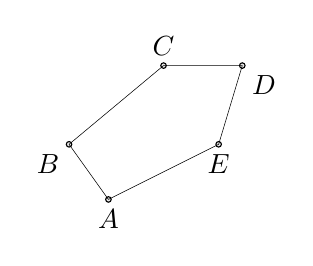
\begin{tikzpicture}
                        \tkzDefPoints{0/0/O, 4/4/L}
                        
                        \tkzDefPoint(1.5,1.3){A}
                        \tkzDefPoint(1,2){B}
                        \tkzDefPoint(2.2,3){C}
                        \tkzDefPoint(3.2,3){D}
                        \tkzDefPoint(2.9,2){E}
                        
                        \tkzLabelPoint[below](A){$A$}
                        \tkzLabelPoint[below left](B){$B$}
                        \tkzLabelPoint[above](C){$C$}
                        \tkzLabelPoint[below right](D){$D$}
                        \tkzLabelPoint[below](E){$E$}
                        
                        \tkzDrawPoints(A,B,C,D,E)
                        \tkzDrawPolygon(A,B,C,D,E)
                    \end{tikzpicture}    
                \end{center}
            \item[Retas:]
                São um conjunto de pontos compreendidos numa linha infinita que não faz curvas e existe em uma dimensão. Retas são ditas concorrentes se tiverem um único ponto em comum. \eg
                \begin{center}
                    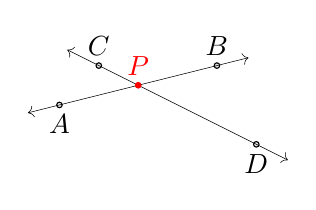
\begin{tikzpicture}
                        \tkzDefPoints{0/0/O, 4/4/L}
                        
                        \tkzDefPoint(1,2){A}
                        \tkzDefPoint(3,2.5){B}
                        \tkzDefPoint(1.5,2.5){C}
                        \tkzDefPoint(3.5,1.5){D}
                        
                        \tkzLabelPoint[below](A){$A$}
                        \tkzLabelPoint[above](B){$B$}
                        \tkzLabelPoint[above](C){$C$}
                        \tkzLabelPoint[below](D){$D$}
                        
                        \tkzDrawPoints(A,B,C,D)
                        \tkzDrawLine[arrows=<->](A,B)
                        \tkzDrawLine[arrows=<->](C,D)

                        \tkzInterLL(A,B)(C,D) \tkzGetPoint{P}
                        \tkzLabelPoint[above, color=red](P){$P$}
                        \tkzDrawPoints[color=red](P)
                    \end{tikzpicture}    
                \end{center}
            \item[Planos:]
                São um conjunto de retas paralelas e perpendiculares postas lado a lado, compreendendo uma forma de duas dimensões. \eg
                \begin{center}
                    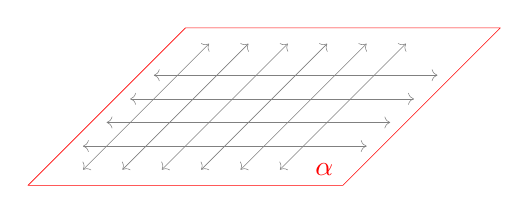
\begin{tikzpicture}
                        \tkzDefPoints{0/0/O, 6/2/L}
                        
                        \tkzDefPoint(0,0){A}
                        \tkzDefPoint(2,2){B}
                        \tkzDefPoint(6,2){C}
                        \tkzDefPoint(4,0){D}
                        
                        \tkzLabelPoint[above left, color=red](D){$\alpha$}
                        
                        \tkzDrawPolygon[color=red](A,B,C,D)

                        \foreach \x in {0.5,1,1.5,2,2.5,3} {
                            \tkzDefPoint(\x,0){P}
                            \tkzDefPoint(\x+2,2){Q}
                            \tkzDrawLine[color=gray, arrows=<->, add = -0.1 and -0.1](P,Q)
                        }
                        \foreach \y in {0.5,0.8,1.1,1.4} {
                            \tkzDefPoint(\y,\y){P}
                            \tkzDefPoint(\y+4,\y){Q}
                            \tkzDrawLine[color=gray, arrows=<->, add = -0.05 and -0.05](P,Q)
                        }
                    \end{tikzpicture}    
                \end{center}
        \end{description}
    %--- 6.1.2
    \subsubsection{Postulados Primitivas}
        \begin{description}
            \item[Existência:] numa reta há infinitos pontos, assim como em um plano;
            \item[Determinação da Reta:] dois pontos distintos determinam uma única reta que passa por eles;
            \item[Determinação do Plano:] três pontos não colineares determinam um único plano que passa por eles;
            \item[Inclusão:] se uma reta tem dois pontos distintos contidos num plano, a reta também está contida nesse mesmo plano.
        \end{description}
    %--- 6.1.3
    \subsubsection{Congruência}
        É uma noção primitiva e intuitiva que expressa uma ideia de semelhança, equivalência ou proporcionalidade.
%------- 6.2
\subsection{Conceitos Básicos}
    %--- 6.2.1
    \subsubsection{Pontos Contidos}
        A definição de estar entre dois pontos obedece aos seguintes postulados:
        \begin{enumerate}
            \item Se P está entre A e B, todos são colineares;
            \item Se P está entre A e B, todos são distintos dois a dois;
            \item Se P está entre A e B, A não está entre P e B, e B não está entre P e A;
            \item Dados quaisquer dois pontos distintos, há um ponto entre eles.
        \end{enumerate}
    %--- 6.2.2
    \subsubsection{Segmento de Reta}
        \begin{description}
            \item[Definição:] é a reunião de dois pontos distintos com o conjunto dos pontos que estão entre eles:
                \[ \overline{AB} = \{ P | \mathring{APB} \} \]
                \begin{center}
                    \begin{tikzpicture}
                        \tkzDefPoints{0/0/O, 6/2/L}
                        
                        \tkzDefPoint(0.4,1.6){A}
                        \tkzDefPoint(1,0.6){B}
                        \tkzDefPoint(3,0.6){C}
                        \tkzDefPoint(2.4,0.6){D}
                        \tkzDefPoint(4,0.6){E}
                        \tkzDefPoint(6,0.6){F}
                        
                        \tkzLabelPoint[below left](A){$A$}
                        \tkzLabelPoint[below](B){$B$}
                        \tkzLabelPoint[below](C){$C$}
                        \tkzLabelPoint[above](D){$D$}
                        \tkzLabelPoint[above](E){$E$}
                        \tkzLabelPoint[below](F){$F$}
                        
                        \tkzDrawPoints(A,B,C,D,E,F)

                        \tkzDrawSegment(A,B)
                        \tkzDrawSegment(B,C)
                        \tkzDrawSegment(D,E)
                        \tkzDrawSegment(E,F)
                    \end{tikzpicture}    
                \end{center}
            \item[Classificação] \hfill
                \begin{description}
                    \item[Consecutivos:] compartilhando uma de suas extremidades. \eg \hfill $\overline{AB},\overline{BC}$;
                    \item[Colineares:] estando contidos numa mesma reta. \eg \hfill $\overline{BC}, \overline{DE}$;
                    \item[Adjacentes:] sendo consecutivos e colineares, mas tendo a extremidade compartilhada como único ponto comum. \eg \hfill $\overline{BC}, \overline{CF}$
                \end{description}
            \item[Postulados de Congruência] \hfill
                \begin{description}
                    \item[Reflexão:] todo segmento é congruente a si mesmo: \[ \overline{AB} \equiv \overline{AB} \]
                    \item[Simetria:] a congruência é estabelecida em ambas as direções de comparação: \[ \overline{AB} \equiv \overline{CD} \leftrightarrow \overline{CD} \equiv \overline{AB} \]
                    \item[Transitividade:] se um primeiro segmento é congruente à um segundo, e este segundo é congruente a um terceiro, o terceito também é congruente ao primeiro: \[ \overline{AB} \equiv \overline{CD} \wedge \overline{CD} \equiv \overline{EF} \rightarrow \overline{AB} \equiv \overline{EF} \]
                    \item[Transporte:] dado um segmento contido numa semirreta, há um único ponto que forma com a origem da semirreta um segmento congruente ao primeiro: \[ \overline{XY} \in \overrightarrow{AB}, \exists ! Z \in \overrightarrow{AB} | \overline{XY} \equiv \overline{AZ} \]
                \end{description}
            \item[Medida] \hfill \\
                A medida de um segmento é um número real positivo que quantifica o seu comprimento:
                \[ m(\overline{AB}) \in \mathbb{R}_{+} | \overline{AB} \equiv \overline{CD} \leftrightarrow m(\overline{AB}) = m(\overline{CD}) \]
            \item[Ponto Médio] \hfill \\
                O ponto médio é um ponto único que divide um segmento em dois segmentos congruentes:
                \[ \exists ! M \in \overline{AB} | \overline{AM} \equiv \overline{MB} \]
            \item[Comparação de Segmentos] \hfill \\
                Dado uma semirreta com um ponto qualquer em seu comprimento, ao inserir um segunto ponto qualquer e comparar os segmentos formados da origem até cada um dos pontos, surgem três possíveis estados:
                \[ \overrightarrow{AX} \ni Y | \begin{dcases} \mathring{AYX} \rightarrow \overline{AX} > \overline{AY} \leftrightarrow m(\overline{AX}) > m(\overline{AY}) \\ X = Y \rightarrow \overline{AX} \equiv \overline{AY} \\ \mathring{AXY} \rightarrow \overline{AX} < \overline{AY} \leftrightarrow m(\overline{AX}) < m(\overline{AY}) \end{dcases} \]
            \item[Distância Métrica] \hfill \\
                A distância métrica entre dois pontos é o comprimento do segmento formado por eles expresso em valor numperico, podendo ser 0.
            \item[Distância Geométrica] \hfill \\
                A distância geométrica entre dois pontos é qualquer segmento congruente ao segmento formado por eles, podendo ser nula.
            \item[Adição] \hfill \\
                A adição de dois segmentos de reta, gera um segmento formado por dois adjacentes e congruentes aos somados:
                \[ \overline{AB} + \overline{CD} = \overline{EF} \leftrightarrow m(\overline{AB}) + m(\overline{CD}) = m(\overline{EF}) \]
        \end{description}
    %--- 6.2.3
    \subsubsection{Semirreta}
        É a reunião de um segmento de reta com o conjunto dos pontos que contém uma das extremidades entre si e a outra extremidade do segmento:
        \[ \overrightarrow{AB} = \overline{AB} \cup \{ P | \mathring{ABP} \} \]
        \begin{center}
            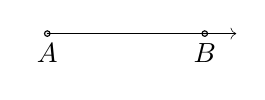
\begin{tikzpicture}
                \tkzDefPoints{0/0/O, 3/2/L}
                
                \tkzDefPoint(1,1){A}
                \tkzDefPoint(3,1){B}
                
                \tkzLabelPoint[below](A){$A$}
                \tkzLabelPoint[below](B){$B$}
                
                \tkzDrawPoints(A,B)

                \tkzDrawSegment[arrows=->, add=0 and 0.2](A,B)
            \end{tikzpicture}    
        \end{center}
    %--- 6.2.4
    \subsubsection{Região}
        Um conjunto de pontos quaisquer pode ser chamado região ou figura, e será classificado como côncavo ou convexo, sendo côncavo quando não convexo, e convexo quando dois pontos distintos quaisquer são extremidades de um segmento de reta inteiramente contido na região, se for unitário, ou se for vazio. \eg
        \begin{center}
            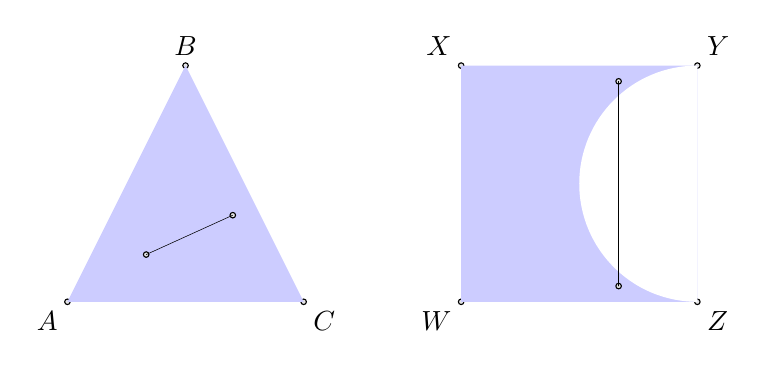
\begin{tikzpicture}
                \tkzDefPoints{0/0/O, 8/3/L}
                
                \tkzDefPoint(0,0){A}
                \tkzDefPoint(1.5,3){B}
                \tkzDefPoint(3,0){C}

                \tkzDefPoint(5,0){W}
                \tkzDefPoint(5,3){X}
                \tkzDefPoint(8,3){Y}
                \tkzDefPoint(8,0){Z}

                \tkzDefPoint(6.5,1.5){U}
                \tkzDefPoint(8,1.5){V}
                
                \tkzLabelPoint[below left](A){$A$}
                \tkzLabelPoint[above](B){$B$}
                \tkzLabelPoint[below right](C){$C$}

                \tkzLabelPoint[below left](W){$W$}
                \tkzLabelPoint[above left](X){$X$}
                \tkzLabelPoint[above right](Y){$Y$}
                \tkzLabelPoint[below right](Z){$Z$}

                \tkzDrawPoints(A,B,C,W,X,Y,Z)
                
                \tkzFillPolygon[fill=blue!20](A,B,C)

                \tkzFillPolygon[fill=blue!20](W,X,Y,Z)
                \tkzFillSector[fill=white](V,Y)(Z)

                \tkzDefPoint(1,0.6){x}
                \tkzDefPoint(2.1,1.1){y}
                \tkzDrawPoints(x,y)
                \tkzDrawSegment(x,y)

                \tkzDefPoint(7,2.8){x}
                \tkzDefPoint(7,0.2){y}
                \tkzDrawPoints(x,y)
                \tkzDrawSegment(x,y)
            \end{tikzpicture}    
        \end{center}
    %--- 6.2.5
    \subsubsection{Semiplano}
        Dado um plano qualquer, uma reta (origem) o cortará em dois semiplanos, nessa caso opostos e abertos, tal que:
        \[ \alpha ' \equiv \alpha '' \]
        \[ \alpha ' \cap \alpha '' = \varnothing \]
        \[ A \in \alpha ', B \in \alpha '' \rightarrow \overline{AB} \cup r \neq \varnothing \]
        \begin{center}
            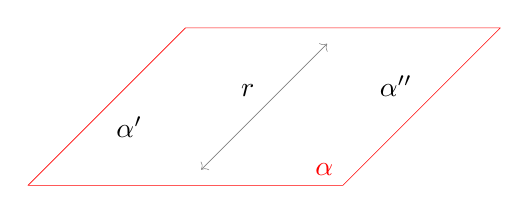
\begin{tikzpicture}
                \tkzDefPoints{0/0/O, 6/2/L}
                
                \tkzDefPoint(0,0){A}
                \tkzDefPoint(2,2){B}
                \tkzDefPoint(6,2){C}
                \tkzDefPoint(4,0){D}
                
                \tkzLabelPoint[above left, color=red](D){$\alpha$}
                
                \tkzDrawPolygon[color=red](A,B,C,D)

                \tkzDefPoint(2,0){P}
                \tkzDefPoint(4,2){Q}
                
                \tkzDrawLine[color=gray, arrows=<->, add = -0.1 and -0.1](P,Q)
                \tkzLabelLine[above left](P,Q){$r$}

                \tkzLabelLine[below right](A,B){$\alpha '$}
                \tkzLabelLine[above left](C,D){$\alpha ''$}
            \end{tikzpicture}    
        \end{center}
    %--- 6.2.6
    \subsubsection{Ângulos}
        \begin{description}
            \item[Definição] \hfill \\
                É a reunião de duas semirretas consecutivas não colineares, onde as semirretas são os lados do ângulo, e a extremidade comum é a origem:
                \[ \hat{\alpha} = \hat{AOB} = \overline{AO} \cup \overline{OB} \]
            \item[Interior] \hfill \\
                O interior do ângulo é a interseção dos semiplanos abertos com origem nos lados do ângulo. Setor angular é a reunião de um ângulo com seu interior.
            \item[Relações] \hfill \\
                Ângulos são consecutivos se compartilham um lado, e adjacentes são consecutivos que não tem nenhum ponto interior em comum. 
                
                Ângulos são ditos opostos pelo vértice quando os lados de um deles são as semirretas opostas aos lados do outro.
            \item[Suplementar Adjacente] \hfill \\
                O suplementar adjacente de um ângulo é formado por um de seus lados e  a semirreta oposta ao seu outro lado.
            \item[Classificação] \hfill \\
                É chamado ângulo reto aquele que é congruente ao seu suplementar adjacente, e agudo e obtuso são respectivamente menores e maiores que um ângulo reto.
            \item[Ângulo Complementar] \hfill \\
                O complementar de um ângulo é a diferença entre ele e um ângulo reto.
                \begin{center}
                    \begin{tikzpicture}
                        \tkzDefPoints{0/0/O, 6/2/L}
                        
                        \tkzDefPoint(0,0){A}
                        \tkzDefPoint(2,0){B}
                        \tkzDefPoint(4,0){C}
                        \tkzDefPoint(6,0){D}
                        \tkzDefPoint(8,0){E}
                        
                        \tkzDefPoint(2,3){P}
                        \tkzDefPoint(4.7,3){Q}
                        \tkzDefPoint(5.3,3){R}

                        \tkzDrawLine[arrows=<->, add = 0 and -0.05](A,E)

                        \tkzDrawSegment(B,P)
                        \tkzDrawSegment(C,Q)
                        \tkzDrawSegment(D,R)

                        \tkzMarkAngle[size=18pt, style=dashed](P,B,A)
                        \tkzMarkAngle[size=18pt](C,B,P)

                        \tkzMarkAngle[size=18pt, style=dashed](Q,C,B)
                        \tkzMarkAngle[size=18pt](D,C,Q)

                        \tkzMarkAngle[size=18pt, style=dashed](R,D,C)
                        \tkzMarkAngle[size=18pt](E,D,R)

                        \tkzLabelAngle[pos=0.3](P,B,A){$\alpha '$}
                        \tkzLabelAngle[pos=0.3](C,B,P){$\alpha$}

                        \tkzLabelAngle[pos=0.3](Q,C,A){$\beta '$}
                        \tkzLabelAngle[pos=0.3](D,C,Q){$\beta$}

                        \tkzLabelAngle[pos=0.4](R,D,C){$\gamma '$}
                        \tkzLabelAngle[pos=0.3](E,D,R){$\gamma$}
                    \end{tikzpicture}    
                \end{center}
            \item[Postulados de Congruência] \hfill \\
                \begin{description}
                    \item[Reflexão:] todo ângulo é congruente a si mesmo:
                        \[ \hat{\alpha} \equiv \hat{\alpha} \]
                    \item[Simetria:] a congruência é estabelecida em ambos os sentidos de comparação:
                        \[ \hat{\alpha} \equiv \hat{\beta} \leftrightarrow \hat{\beta} \equiv \hat{\alpha} \]
                    \item[Transitividade:] se um primeiro ângulo é congruente à um segundo, e este segundo é congruente a um terceiro, o terceito também é congruente ao primeiro:
                        \[ \hat{\alpha} \equiv \hat{\beta} \wedge \hat{\beta} \equiv \hat{\gamma} \rightarrow \hat{\alpha} \equiv \hat{\gamma} \]
                    \item[Transporte:] dado um ângulo e uma semirreta contida num plano, existe uma única outra semirreta consecutiva que forma um ângulo congruente ao primeiro:
                        \[ \hat{AOB} \in \alpha , \overrightarrow{PC} \in \alpha \rightarrow \exists ! \overrightarrow{PD} | \hat{AOB} \equiv \hat{CPD} \]
                \end{description}
            \item[Bissetriz] \hfill \\
                A bissetriz de um ângulo é a semirreta interna a ele que o divide em dois ângulos adjacentes e congruentes.
            \item[Amplitude] \hfill \\
                A amplitude de um ângulo é a medida numérica que o descreve. As principais unidades de medida são o grau (dividido em minutos e segundos), o grado (dividido em centigrado e decimiligrado) e o radiano:
                \[ m(\hat{\alpha}) \in \mathbb{R}_{+} | \hat{\alpha} \equiv \hat{\beta} \leftrightarrow m(\hat{\alpha}) = m(\hat{\beta}) \]
                \[ \gamma = \text{ângulo reto} \]
                \[ 1^{\circ} = \frac{\gamma}{90}, 1' = \frac{1^{\circ}}{60}, 1'' = \frac{1'}{60} \]
                \[ 1^g = \frac{\gamma}{100}, 1^{gg} = \frac{1^g}{100}, 1^{ggg} = \frac{1^gg}{100} \]
                \[ 1^{rad} = \frac{2\gamma}{\pi} \]
            \item[Comparação] \hfill \\
                Dados dois ângulos num mesmo semiplano, com o primeiro tendo um lado compreendido em sua origem, podemos movimentar um ponto que forma um ângulo com a origem do primeiro, e a partir de sua comparação, surgem três possíveis estados:
                \[ \overrightarrow{AB} \in \alpha , \hat{AOB} \in \alpha' , \hat{AOC} \in \alpha' | \begin{dcases} \overrightarrow{OC} \in \hat{AOB} \rightarrow \hat{AOB} > \hat{AOC} \leftrightarrow m(\hat{AOB}) > m(\hat{AOC}) \\ \overrightarrow{OC} = \overrightarrow{OB} \rightarrow \hat{AOB} \equiv \hat{AOC} \\ \overrightarrow{OC} \notin \hat{AOB} \rightarrow \hat{AOB} < \hat{AOC} \leftrightarrow m(\hat{AOB}) < m(\hat{AOC})  \end{dcases} \]
            \item[Adição] \hfill \\
                A adição de dois ângulos, gera um formado por dois adjacentes congruentes aos somados:
                \[ \hat{\alpha} + \hat{\beta} = \hat{\gamma} \leftrightarrow m(\hat{\alpha}) + m(\hat{\beta}) = m(\hat{\gamma}) \]
        \end{description}
%--- 6.3
\subsection{Retas no Plano}
    %--- 6.3.1
    \subsubsection{Relações entre Retas}
        \begin{description}
            \item[Paralelas] \hfill \\
                Duas retas são paralelas quando coincidentes ou quando coplanares e sem pontos em comum:
                \[ r \parallel s \leftrightarrow \begin{dcases} r = s \\ \alpha \supset r,s | r \cup s = \emptyset \end{dcases} \]
            \item[Concorrentes] \hfill \\
                Duas retas são concorrentes quando coplanares e com exatamente um ponto em comum:
                \[ r \nparallel s \leftrightarrow \alpha \subset r, s | \exists!P \in r \cup s \]
            \item[Perpendiculares] \hfill \\
                Duas retas são perpendiculares quando concorrentes formando um ângulo reto
                \[ r \bot s \leftrightarrow r \cap s = P \wedge \hat{r_1Ps_1} = \hat{r_2Ps_2} \]
            \item[Oblíquas] \hfill \\
                Duas retas são oblíquas quando concorrentes e não perpendiculares
        \end{description}
    %--- 6.3.2
    \subsubsection{Postulados}
        \begin{description}
            \item[Existência da Paralela] \hfill \\
                Se duas retas coplanares distintas e uma transversal determinam ângulos alternos congruentes, então essas duas retas são paralelas. \eg
                \begin{center}
                    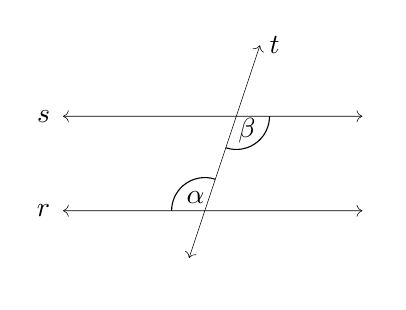
\begin{tikzpicture}
                        \tkzDefPoints{0/0/O, 6/2/L}
                        
                        \tkzDefPoint(0,0.9){A}
                        \tkzDefPoint(4,0.9){B}
                        \tkzDrawLine[arrows=<->, add = 0 and -0.05](A,B){r}
                        \tkzLabelLine[left, pos=-0.01](A,B){$r$}
                        \tkzDefPointOnLine[pos=0.45](A,B)\tkzGetPoint{P}
                        
                        \tkzDefPoint(0,2.1){C}
                        \tkzDefPoint(4,2.1){D}
                        \tkzDrawLine[arrows=<->, add = 0 and -0.05](C,D){s}
                        \tkzLabelLine[left, pos=-0.01](C,D){$s$}
                        \tkzDefPointOnLine[pos=0.55](C,D)\tkzGetPoint{Q}

                        \tkzDefPoint(2.5,3){E}
                        \tkzDefPoint(1.5,0){F}
                        \tkzDrawLine[arrows=<->, add = 0 and -0.1](E,F){t}
                        \tkzLabelLine[right, pos=0](E,F){$t$}

                        \tkzMarkAngle[size=12pt](Q,P,A)
                        \tkzLabelAngle[pos=0.2](Q,P,A){$\alpha$}

                        \tkzMarkAngle[size=12pt](P,Q,D)
                        \tkzLabelAngle[pos=0.23](P,Q,D){$\beta$}
                    \end{tikzpicture}    
                \end{center}
                \[ \alpha \equiv \beta \therefore r \parallel s \]
            \item[Unicidade da Paralela] \hfill \\
                Por um ponto passa uma única reta paralela a uma reta dada
            \item[Existência e Unicidade da Perpendicular] \hfill \\
                Por um ponto qualquer fora de uma reta dada, existe uma e somente uma reta perpendicular a reta dada
        \end{description}
    %--- 6.3.3
    \subsubsection{Projeção}
        \begin{description}
            \item[Ortogonal] \hfill \\
                Chama-se projeção ortogonal de um ponto sobre uma reta o ponto de interseção da reta com sua perpendicular conduzida ao ponto
            \item[Segmento sobre reta] \hfill \\
                A projeção de um segmento sobre uma reta não perpendicular é o segmento formado pela projeção dos pontos que formam o primeiro segmento
        \end{description}
    %--- 6.3.4
    \subsubsection{Teorema de Thales}
        \begin{description}
            \item[Conceitos Iniciais:] \hfill \\
                \begin{itemize}
                    \item[$\bullet$] Feixe de retas paralelas é um conjunto de retas coplanares paralelas entre si;
                    \item[$\bullet$] Uma transversal dos feixes é uma reta transversal a todas as retas do feixe de paralelas;
                    \item[$\bullet$] Pontos correspondentes são pontos de transversais cortados por uma mesma reta do feixe;
                    \item[$\bullet$] Segmentos correspondentes são segmentos formados por pontos respectivamente correspondentes.
                \end{itemize}
            \item[Teorema:] \hfill \\
                Se duas retas são transversais de um feixe de retas paralelas, então a razão entre dois segmentos quaisquer de uma delas é igual a razão entre os respectivos segmentos correspondentes da outra. \eg
                \begin{center}
                    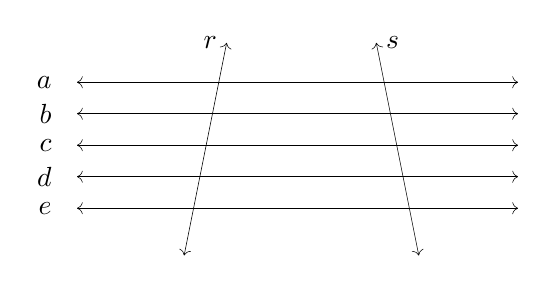
\begin{tikzpicture}
                        \tkzDefPoints{0/0/O, 6/3/L}
                        
                        \tkzDefPoint(0,0.4){X}
                        \tkzDefPoint(4,0.4){Y}
                        \tkzDrawLine[arrows=<->](X,Y){e}
                        \tkzLabelLine[left, pos=-0.25](X,Y){$e$}

                        \tkzDefPoint(0,0.8){X}
                        \tkzDefPoint(4,0.8){Y}
                        \tkzDrawLine[arrows=<->](X,Y){d}
                        \tkzLabelLine[left, pos=-0.25](X,Y){$d$}

                        \tkzDefPoint(0,1.2){X}
                        \tkzDefPoint(4,1.2){Y}
                        \tkzDrawLine[arrows=<->](X,Y){c}
                        \tkzLabelLine[left, pos=-0.25](X,Y){$c$}

                        \tkzDefPoint(0,1.6){X}
                        \tkzDefPoint(4,1.6){Y}
                        \tkzDrawLine[arrows=<->](X,Y){b}
                        \tkzLabelLine[left, pos=-0.25](X,Y){$b$}

                        \tkzDefPoint(0,2){X}
                        \tkzDefPoint(4,2){Y}
                        \tkzDrawLine[arrows=<->](X,Y){a}
                        \tkzLabelLine[left, pos=-0.25](X,Y){$a$}

                        \tkzDefPoint(1.1,2.5){X}
                        \tkzDefPoint(0.5,-0.5){Y}
                        \tkzDrawLine[arrows=<->, add = 0 and -0.1](X,Y){r}
                        \tkzLabelLine[left, pos=0](X,Y){$r$}

                        \tkzDefPoint(3,2.5){X}
                        \tkzDefPoint(3.6,-0.5){Y}
                        \tkzDrawLine[arrows=<->, add = 0 and -0.1](X,Y){s}
                        \tkzLabelLine[right, pos=0](X,Y){$s$}
                    \end{tikzpicture}    
                \end{center}
                \[ A = r \cup a, B = r \cup c, C = r \cup e \]
                \[ A' = s \cup a, B' = s \cup c, C' = s \cup e \]
                \[ \frac{\overline{AB}}{\overline{AC}} = \frac{\overline{A'B'}}{\overline{A'C'}} \]
        \end{description}
    %--- 6.3.5
    \subsubsection{Mediatriz}
        A mediatriz de um segmento de reta é a reta perpendicular ao segmento pelo seu ponto médio
        \begin{center}
            \begin{tikzpicture}
                \tkzDefPoints{0/0/O, 3/2/L}
                
                \tkzDefPoint(0,1){A}
                \tkzDefPoint(2,1){B}
                \tkzDefPoint(1,1){M}
                
                \tkzLabelPoint[below](A){$A$}
                \tkzLabelPoint[below](B){$B$}
                \tkzLabelPoint[below right](M){$M$}
                
                \tkzDrawPoints(A,B,M)

                \tkzDrawSegment[add=0 and 0](A,B)

                \tkzDefPoint(1,2){X}
                \tkzDefPoint(1,0){Y}
                \tkzDrawLine[arrows=<->](X,Y){m}
                \tkzLabelLine[left, pos=0](X,Y){$m$}
            \end{tikzpicture}
        \end{center}
%------- 6.4
\subsection{Polígonos}
    %--- 6.4.1
    \subsubsection{Definição}
        Chama-se polígono a reunião dos segmentos formados por três ou mais pontos distintos onde dois consecutivos não são colineares. \eg:
        \[ \Diamond ABCDE = \overline{AB} \cup \overline{BC} \cup \overline{CD} \cup \overline{DE} \cup \overline{EA} \]
        \begin{center}
            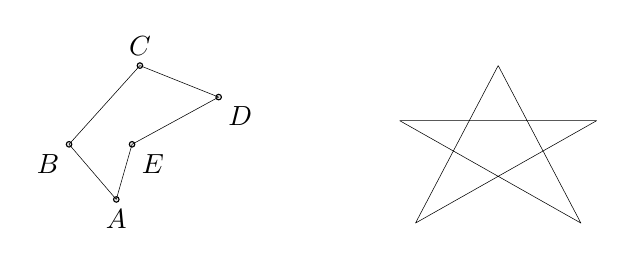
\begin{tikzpicture}
                \tkzDefPoints{0/0/O, 9/3.5/L}
                
                \tkzDefPoint(1.9,1.3){A}
                \tkzDefPoint(1.3,2){B}
                \tkzDefPoint(2.2,3){C}
                \tkzDefPoint(3.2,2.6){D}
                \tkzDefPoint(2.1,2){E}
                
                \tkzLabelPoint[below](A){$A$}
                \tkzLabelPoint[below left](B){$B$}
                \tkzLabelPoint[above](C){$C$}
                \tkzLabelPoint[below right](D){$D$}
                \tkzLabelPoint[below right](E){$E$}

                \tkzDefPoint(5.7,1){F}
                \tkzDefPoint(8,2.3){G}
                \tkzDefPoint(5.5,2.3){H}
                \tkzDefPoint(7.8,1){I}
                \tkzDefPoint(6.75,3){J}
                
                \tkzDrawPoints(A,B,C,D,E)
                \tkzDrawPolygon(A,B,C,D,E)
                \tkzDrawPolygon(F,G,H,I,J)
            \end{tikzpicture}    
        \end{center}
    %--- 6.4.2
    \subsubsection{Composição Nominal dos Elementos}
        \begin{description}
            \item[Superfície Poligonal] \hfill \\
                Superfície Poligonal, também chamada de área ou região poligonal, é a reunião do polígono com seu interior;
            \item[Vértices] \hfill \\
                Vértices são os pontos que formam a região que define o polígono;
            \item[Lados] \hfill \\
                Os lados são os segmentos de reta formados ordenadamente pelos vértices do polígono;
            \item[Ângulos] \hfill \\
                Ângulos internos são aqueles cujo interior coincide com a região do polígono, enquanto os ângulos externos são os suplementares aos internos;
            \item[Perímetro] \hfill \\
                O perímetro é a soma das distâncias métricas dos lados do polígono, enquanto e semiperímetro é a metade do perímetro;
            \item[Diagonal] \hfill \\
                Uma diagonal é um segmento de reta cujas extremidades são vértices não consecutivos do polígono.
        \end{description}
    %--- 6.4.3
    \subsubsection{Nomenclatura}
        \begin{description}
            \item[Quanto a Forma] \hfill \\
                Um polígono será classificado como simples ou complexo, e côncavo ou convexo de acordo com a sua forma:
                \begin{itemize}
                    \item[$\bullet$] O polígono simples é aquele cuja interseção de quaisquer dois lados não consecutivos é vazia, e complexo em caso contrário;
                    \item[$\bullet$] O polígono é convexo quando a reta determinada por quaisquer dois vértices consecutivos inclui todos os outros no interior do semiplano que ela determina.
                \end{itemize} 
            \item[Quanto ao Número de Lados] \hfill \\
                Os polígonos recebem nomes específicos de acordo com o seu número de lados:
                \begin{enumerate}[start=3]
                    \begin{multicols}{3}
                        \item Triângulo
                        \item Quadrilátero
                        \item Pentágono
                        \item Hexágono
                        \item Heptágono
                        \item Octógono
                        \item Eneágono
                        \item Decágono
                        \item Undecágono
                        \item Dodecágono
                        \item Tridecágono
                        \item Tetradecágono
                        \item Pentadecágono
                        \item Hexadecágono
                        \item Heptadecágono
                        \item Octodecágono
                        \item Eneadecágono
                        \item Icoságono
                        \setcounter{enumi}{29}
                        \item Triacontágono
                        \setcounter{enumi}{39}
                        \item Tetracontágono
                        \setcounter{enumi}{49}
                        \item Pentacontágono
                        \setcounter{enumi}{59}
                        \item Hexacontágono
                        \setcounter{enumi}{69}
                        \item Heptacontágono
                        \setcounter{enumi}{79}
                        \item Octacontágono
                        \setcounter{enumi}{89}
                        \item Eneacontágono
                        \setcounter{enumi}{99}
                        \item Hectacontógono
                    \end{multicols}
                \end{enumerate}

                Equanto os demais polígonos com mais de vinte e menos de cem lados tem seus nomes compostos pela seguinte regra:
                \begin{center}
                    \begin{tabular}{|cc|c|cc|c|}
                            \hline
                            \multicolumn{2}{|c|}{\multirow{2}{3em}{\textbf{Dezena}}} & \textbf{Junção} & \multicolumn{2}{c|}{\textbf{Unidade}} & \textbf{Sufixo} \\
                            && \multirow{9}{1em}{cai} & \textbf{1} & ena & \multirow{9}{2em}{gono} \\
                            \textbf{20} & Icosi && \textbf{2} & di &\\
                            \textbf{30} & Triaconta && \textbf{3} & tri &\\
                            \textbf{40} & Tetraconta && \textbf{4} & tetra &\\
                            \textbf{50} & Pentaconta && \textbf{5} & penta &\\
                            \textbf{60} & Hexaconta && \textbf{6} & hexa &\\
                            \textbf{70} & Heptaconta && \textbf{7} & hepta &\\
                            \textbf{80} & Octaconta && \textbf{8} & octa &\\
                            \textbf{90} & Eneaconta && \textbf{9} & enea &\\
                            \hline
                    \end{tabular}
                \end{center}
            \item[Quanto a Congruência de Seus Lados] \hfill \\
                Um polígono pode ser classificado como equiângulo, quando possui todos os ângulos congruentes, e equilátero, quando possui todos os lados congruentes. Um polígono convexo simultaneamente equilátero e equiângulo é chamado regular.
        \end{description}
    %--- 6.4.4
    \subsubsection{Descrição Matemática dos Elementos}
        \begin{description}
            \item[Diagonais] \hfill \\
                O número de diagonais de um polígono é proporcional ao seu número de lados:
                \[ d = \frac{n(n-3)}{2} \]
            \item[Ângulos Internos] \hfill \\
                A soma dos ângulos internos de um polígono convexo é proporcional ao seu número de lados:
                \[ S_i = (n-2) \cdot \pi^{rad} \]
            \item[Ângulos Externos] \hfill \\
                A soma dos ângulos externos de um polígono tem o valor constante de quatro ângulos retos:
                \[ S_e = 2\pi^{rad} \]
        \end{description}
%------- 6.5
\subsection{Polígonos Regulares}
    %--- 6.5.1
    \subsubsection{Inscrição e Circunscrição}
        Ao se dividir uma circunferência em $n$ arcos congruentes, formam-se dois polígonos regulares:
        \begin{description}
            \item[Inscrito:] reunindo as cordas determinadas por dois pontos de divisão consecutivos, é desenhado um polígono regular de $n$ lados inscrito na circunferência;
            \item[Circunscrito:] reunindo as tangentes traçadas aos pontos de divisão, é desenhado um polígono regular de $n$ lados circunstrito à circunferência.
        \end{description}
        
        Em decorrência dessa propriedade, denota-se que todo polígono regular é inscritível em exatamente uma circunferência, e é circunscritível a exatamente uma circunferência.
    %--- 6.5.2
    \subsubsection{Elementos Notáveis}
        \begin{description}
            \item[Centro:] é o centro comum das circunferências inscrita e circunscrita;
            \item[Raio:] é a distância do centro até um vértice, e portanto o raio da circunferência inscrita;
            \item[Apótema:] é a distância do centro até o ponto médio de um lado, e portanto o raio da circunferência circunscrita;
            \item[Diagonal Principal:] existente apenas no caso de um número par de lados, é definida pela diagonal que atravessa o centro;
            \item[Maior Diagonal:] é a maior distância entre dois vértices, sendo a diagonal principal quando aplicável;
            \item[Menor Diagonal:] é a menor distância entre dois vértices.
        \end{description}
    %--- 6.5.3
    \subsubsection{Descrição Matemática dos Elementos}
        \begin{description}
            \item[Raio]
                \[ R = \frac{l}{2\sin{\frac{\pi}{n}}} \]
            \item[Lado]
                \[ l_{2n} = \sqrt{R \cdot (2R-\sqrt{4R^2 - l^2_n})} \]
                \begin{multicols}{3}
                    \noindent\[ l_3 = R\sqrt{3} \]
                    \[ l_4 = R\sqrt{2} \]
                    \[ l_5 = \frac{R\sqrt{10 - 2\sqrt{5}}}{2} \]
                \end{multicols}
            \item[Apótema]
                \[ r = \frac{\sqrt{4R^2 - l^2}}{2} = \frac{l}{2\tan{\frac{\pi}{n}}} = R \cdot \cos{\frac{\pi}{2}} \]
                \begin{multicols}{2}
                    \noindent\[ r_3 = \frac{R}{2} \]
                    \[ r_4 = \frac{R\sqrt{2}}{2} \]
                    \[ r_5 = \frac{R + R\sqrt{5}}{4} \]
                    \[ r_6 = \frac{R\sqrt{3}}{2} \]
                \end{multicols}
            \item[Número de Diagonais por Vértice] \hfill \\
                \[ d_n = (n-3) \]
            \item[Número de Diagonais Únicas] \hfill \\
                \[ dt_n = \frac{n \cdot d_n}{2} \]
            \item[Diagonal Principal] \hfill \\
                \[ d_p = 2R \]
            \item[Maior Diagonal]
                \[ d_M = \frac{r + R}{\sin{\frac{\hat{\alpha_i}(n-1)}{2(n-2)}}} | n > 3 \]
            \item[Menor Diagonal]
                \[ d_m = \frac{l \cdot \sin{\hat{\alpha_i}}}{\sin{\frac{\hat{\alpha_i}}{n-2}}} | n > 3 \]
            \item[Semiperímetro]
                \[ p = \frac{ n \cdot l}{2} \]
            \item[Área]
                \[ A = \frac{n \cdot l^2}{4\tan{\frac{\pi}{n}}} = p \cdot r \]
            \item[Circunferência Inscrita] \hfill \\
                \begin{multicols}{2}
                    \noindent\[ C = \frac{\pi \cdot l}{\tan{\frac{\pi}{n}}} \]
                    \[ A = \frac{\pi \cdot l^2}{4\tan^2{\frac{\pi}{n}}} \]
                \end{multicols}
            \item[Circunferência Circunscrita] \hfill \\
                \begin{multicols}{2}
                    \noindent\[ C = \frac{\pi \cdot l}{\sin{\frac{\pi}{n}}} \]
                    \[ A = \frac{\pi \cdot l^2}{4\sin^2{\frac{\pi}{n}}} \]
                \end{multicols}
        \end{description}
%------- 6.6
\subsection{Triângulos}
    %--- 6.6.1
    \subsubsection{Descrição Matemática}
        \begin{center}
            \begin{tikzpicture}
                
            \end{tikzpicture}
        \end{center}
        \begin{description}
            \item[Condição de Existência:] \hfill \\
            \item[Área:] \hfill \\
            \item[Lados:] \hfill \\
            \item[Altura:] \hfill \\
            \item[Mediatriz e Circuncentro:] \hfill \\
            \item[Mediana e Baricentro:] \hfill \\
            \item[Bissetriz e Incentro:] \hfill \\
            \item[Círculo de 9 Pontos e Reta de Euler:] \hfill \\
        \end{description}
    %--- 6.6.2
    \subsubsection{Classificação}
        Quanto aos lados:
        \begin{description}
            \item[Equilátero:] Composto por três lados congruentes;
            \item[Isósceles:] Composto por exatamente dois lados congruentes;
            \item[Escaleno:] Composto por três lados não congruentes entre si.
        \end{description}
        
        Quanto aos ângulos:
        \begin{description}
            \item[Retângulo:] Contêm exatamente um ângulo reto;
            \item[Obtusângulo:] Contêm exatamente um ângulo obtuso;
            \item[Acutângulo:] Contêm todos os três ângulos agudos.
        \end{description}
    %--- 6.6.3
    \subsubsection{Congruência}
        \begin{description}
            \item[Definição] \hfill \\
                Um triângulo é congruente a outro quando é possível estabelecer uma correspondência entre seus vértices de modo que, seus lados e seus ângulos sejam ordenadamente congruentes:
                \[ \triangle ABC \equiv \triangle XYZ \leftrightarrow \begin{dcases} \overline{AB} \equiv \overline{XY} \hphantom{-} \hphantom{"^"} \hphantom{-} \hat{ABC} \equiv \hat{XYZ} \\ \overline{BC} \equiv \overline{YZ} \hphantom{-} \wedge \hphantom{-} \hat{BCA} \equiv \hat{YZX} \\ \overline{AC} \equiv \overline{XZ} \hphantom{-} \hphantom{"^"} \hphantom{-} \hat{CAB} \equiv \hat{ZXY} \end{dcases} \]
            \item[Casos de Congruência] \hfill \\
                \begin{description}
                    \item[LAL]: Ordenadamente congruentes dois lados e o ângulo compreendido entre eles;
                    \item[ALA]: Ordenadamente congruentes um lado e os dois ângulos a ele adjacentes;
                    \item[LLL]: Ordenadamente congruentes os três lados;
                    \item[LAAo]: Ordenadamente congruentes um lado, seu ângulo oposto e um ângulo congruente.
                \end{description}
        \end{description}
    %--- 6.6.
    \subsubsection{}
    %--- 6.6.
    \subsubsection{}
%------- 6.7
\subsection{Quadriláteros Notáveis}
%------- 6.8
\subsection{Circunferências}
    %------- ------- 7
    \section{Trigonometria}
    %------- 7.1
\subsection{Calor e Temperatura}
    \[ \Upsilon \pi o \mu o \nu \eta \]
%------- 7.2
\subsection{Leis da Termodinâmica}
    \[ \Upsilon \pi o \mu o \nu \eta \]
    %------- ------- 8
    \section{Geometria Analítica}
    \[ \Upsilon \pi o \mu o \nu \eta \]
    %------- ------- 9
    \section{Geometria Espacial}
    %------- 9.
\subsection{Ótica Geométrica}
    \[ \Upsilon \pi o \mu o \nu \eta \]
%------- 9.
\subsection{Interferência}
    \[ \Upsilon \pi o \mu o \nu \eta \]
%------- 9.
\subsection{Difração}
    \[ \Upsilon \pi o \mu o \nu \eta \]
%------- 9.
\subsection{Polarização}
    \[ \Upsilon \pi o \mu o \nu \eta \]
    %------- ------- 10
    \section{Matemática Discreta}
    \[ \Upsilon \pi o \mu o \nu \eta \]
    %------- ------- 11
    \section{Matemática Aplicada}
    %------- 11.1
\subsection{Matemática Financeira}
    %--- 11.1.1
    \subsubsection{Introdução}
        Ao lidar com expressões monetárias, o valor a ser tratado é chamado de capital; A correção do capital para o caso de investimento ou empréstimo é chamado juros; A correção do capital expressa em porcentagem sobre determinado período de tempo é chamada taxa de juros; O valor do capital em determinado tempo após aplicados os juros é chamado montante:
        \[ J = C \cdot i \]
        \[ M = C + J \]
    %--- 11.1.2
    \subsubsection{Variação Percentual}
        Para o caso de uma mudança sobre uma determinada grandeza em um espaço de tempo, a variação percentual é a razão entre a diferença e o valor inicial expressa em porcentagem:
        \[ \Delta V = \frac{V_t - V_0}{V_0} = \frac{V_t}{V_0} - 1 \]
        Quando consideradas mudanças sucessivas em determinados espaços de tempo, o cálculo da variação percentual acumulada é feito da seguinte forma:
        \[ \Delta V_n = \frac{V_n - V_{n-1}}{V_{n-1}} \]
        \[ V_n = V_0 \displaystyle\prod_{i=0}^{n} {1 + \Delta V_i} \]
    %--- 11.1.3
    \subsubsection{Inflação e Deflação}
        A inflação e a deflação são sentidos opostos do movimento sobre o valor real de uma moeda em relação a determinado padrão, sendo respectivamente a desvalorização e a valorização da moeda.
    %--- 11.1.4
    \subsubsection{Regimes de Capitalização}
        \begin{description}
            \item[Capitalização Simples:]
                No regime de capitalização simples, os juros incidem sobre as parcelas com sua taxa aplicada sobre o capital inicial:
                \[ J = C \cdot i \cdot t \]
            \item[Capitalização Composta:]
                No regime de capitalização composta, os juros incidem sobre as parcelas com sua taxa aplicada sobre o montante de cada parcela:
                \[ M_t = C \cdot \displaystyle\prod_{n=1}^{t} {1 + i_n} = C \cdot (1 + i_1) \cdots (1 + i_t) \]
                Considerando que a taxa de juros se mantenha inalterada com o passar do tempo:
                \[ M_t = C \cdot (1+i)^t \]
                Quando necessário calcular o valor atual a partir do valor futuro, basta inverter os juros de volta:
                \[ C = \frac{M_t}{(1+i)^t} \]
        \end{description}
    %--- 11.1.5
    \subsubsection{Sequência Uniforme de Pagamentos}
        Dado um valor financiado em parcelas iguais sob um regime de capitalização composta com taxa de juros fixa, a sequência das parcelas forma uma progressão geométrica. O valor atual do financiamento é dado pela soma dos valores atuais das parcelas:
        \[ C = \displaystyle\sum_{n=1}^{t} {\frac{V_p}{(1+i)^n}} = V_p \cdot \frac{(1+i)^t - 1}{(1+i)^t \cdot i} \]
    %--- 11.1.6
    \subsubsection{Sequência Uniforme de Depósitos}
        Considerando uma sequência de depósitos iguais sob um regime de capitalização composta com taxa de juros fixa, a sequência dos depósitos forma uma progressão geométrica. O montante depositado em dado momento é dado pela soma dos valores atuais dos depósitos:
        \[ C = \displaystyle\sum_{n=1}^{t-1} {V_d \cdot (1+i)^n} = V_d \cdot \frac{(1+i)^t -1}{i} \]
%------- 11.2
\subsection{Estatística}
    %--- 11.2.1
    \subsubsection{Introdução}
        Estatística é a aplicação da probabilística para explicar a frequência de eventos em situações observacionais e modelar a incerteza para prever eventos futuros. Divide-se em:
        \begin{description}
            \item[Amostragem:] a população é o conjunto de objetos que interessam ao estudo e uma amostra é um subconjunto da população formado por um procedimento definido, os elementos desse subconjunto são os pontos amostrais;
            \item[Estatística Descritiva:] é a técnica de organização e descrição dos dados coletados do espaço amostral;
            \item[Estatística Inferencial:] é a realização de inferências ou modelagens a partir dos dados do espaço amostral.
        \end{description}
    %--- 11.2.2
    \subsubsection{Variáveis}
        São características dos elementos do espaço amostral que adquirem determinado valor, sendo classificadas em:
        \begin{description}
            \item[Qualitativas:] são atributos ou aspectos nominais, não podendo ser numericamente mensurados. e.g.: gênero, estado civil, religião;
            \item[Quantitativas:] são valores numericamente mensuráveis, divididas em:
                \begin{description}
                    \item[discretas - ] são obtidas por contagem e representadas como elementos de um conjunto finito e mensurável. \eg \ frequência semanal;
                    \item[contínuas - ] são obtidas por mensuração, se expressando por valores pertencentes a um intervalo real. \eg \ idade, renda familiar;
                \end{description}
        \end{description}
    %--- 11.2.3
    \subsubsection{Frequência}
        Para cada variável estudada, conta-se o número de ocorrências total de cada valor para se obter a frequência absoluta, e ao dividir o número de ocorrências de um determinado valor pela frequência absoluta, obtém-se a frequência relativa daquela ocorrência. \eg
        \[ x_1 = 16, x_2 = 14, x_3 = 9 \]
        \[ f_x = 39, f_{x_1} = \frac{16}{39} \]
    %--- 11.2.4
    \subsubsection{Medidas de Centralidade}
        \begin{description}
            \item[Média Aritmética Simples:]
                Definida pelo somatório dos valores assumidos pela variável dividido pelo número de valores:
                \[ \overline{x} = \displaystyle\sum_{i=1}^{n} {x_i \cdot n^{-1}} = \frac{x_1 + \cdots + x_n}{n} \]
            \item[Média Aritmética Ponderada:]
                Definida pelo somatório dos produtos dos valores assumidos pela varíavel por seus respectivos pesos (comunmente sua frequência relativa) divido pelo somatório dos pesos:
                \[ \overline{x} = \frac{\displaystyle\sum_{i=1}^{n} {x_i \cdot p_i}}{\displaystyle\sum_{i=1}^{n} {p_i}} = \frac{x_1 \cdot p_1 \cdots x_n \cdot p_n}{p_1 + \cdot + p_n} \]
            \item[Média Geométrica:]
                Definida pela raiz do produto dos valores assumidos pela variável:
                \[ G_x = \left(\displaystyle\prod_{i=1}^{n} {x_n}\right)^{\frac{1}{n}} = \sqrt[n]{x_1 \cdots x_n} \]
            \item[Média Harmônica:]
                Definida pelo inverso da média aritmética dos inversos dos valores assumidos pela variável:
                \[ H_x = \left(\displaystyle\sum_{i=1}^{n} {\frac{x_{i}^{-1}}{n}}\right)^{-1} = \left(\frac{x_1^{-1} + \cdots + x_n^{-1}}{n}\right)^{-1} \]
            \item[Mediana:]
                É o valor que separa as metades maior e menor dos valores assumidos por uma variável quando em ordem crescente, sendo o termo do meio em um número ímpar de valores ou a média dos 2 termos do meio:
                \[ x = \{ x_i \ | \ x_i \leq x_{i+1} \ \forall i \in \mathbb{N}^n \} \]
                \[ Me = \begin{dcases} x_{\frac{n+1}{2}} \rightarrow \frac{n}{2} \notin \mathbb{N} \\ \overline{x_\frac{n}{2},x_{\frac{n}{2}+1}} \rightarrow \frac{n}{2} \in \mathbb{N} \end{dcases} \]
            \item[Moda:]
                É o valor com a maior frequência relativa dentre os possíveis valores da variável:
                \[ Moda_x = x_i \ | \ f_{x_i} \geq f_{x_j} \ \forall j \in \mathbb{N}^n - i \]
        \end{description}
    %--- 11.2.5
    \subsubsection{Medidas de Dispersão}
        \begin{description}
            \item[Amplitude:]
                É a diferença entre o maior e o menor valor de uma variável,
            \item[Variância:]
                Indica a distância de cada valor da média dos valores possíveis da variável. É definida pela média dos quadrados das diferenças entre cada valor e a média aritmética da variável:
                \[ \sigma^2 = \displaystyle\sum_{i=1}^{n} {(x_i - \overline{x})^2 \cdot n^{-1}}  \]
            \item[Desvio Padrão:]
                Definido pela raiz quadrada da variância:
                \[ \sigma = \sqrt{\sigma^2} \]
            \item[Desvio Médio:]
                Definido pela média dos módulos das diferenças entre cada valor e a média aritmética da variável:
                \[ Dm_x = \displaystyle\sum_{i=1}^{n} {|x_i - \overline{x}| \cdot n^{-1}} \]
        \end{description}
    %--- 11.2.6
    \subsubsection{Medidas de Posição}
        \begin{description}
            \item[Quartis:] divide os valores assumidos pela variável em 4 setores iguais;
            \item[Decis:] divide os valores assumidos pela variável em 10 setores iguais;
            \item[Percentis:] aponta o limiar que separa os valores assumidos pela variável na porcentagem indicada, onde tal porcentagem dos valores são menores ou iguais a ele.
        \end{description}
    %--- 11.2.7
    \subsubsection{Inferência Bayesiana}
        \[ \Upsilon \pi o \mu o \nu \eta \]
    %------- ------- 12
    \section{Cálculo e Análise}
    %------- 12.1
\subsection{Limite}
%------- 12.2
\subsection{Derivada}
%------- 12.3
\subsection{Integral}
    %------- ------- 13
    \section{Constantes da Matemática}
    %------- 13.1
\subsection{Raiz Quadrada de Dois}
%------- 13.2
\subsection{Pi}
%------- 13.3
\subsection{Proporção Áurea}
%------- 13.4
\subsection{Unidade Imaginária}
%------- 13.5
\subsection{Número de Euler}
%------- 13.6
\subsection{Constante de Euler-Mascheroni}
    %------- ------- 14
    \section{Funções Definidas}
    %------- 14.1
\subsection{Série de Taylor}
%------- 14.2
\subsection{Função Zeta de Riemann}
%------- 14.3
\subsection{Série de Dirichlet}
%------- 14.4
\subsection{Função de Gauss}
%------- 14.5
\subsection{Função Gama}
%------- ------- ------- End of Document
\end{document}